\documentclass[12pt,
			 oneside,
			 %draft
             ]{UAHMemoir}
             
\author{Aldo Borrero González}
\title{Gestión dinámica de grupos en una plataforma de aprendizaje virtual basada en TikiWiki}

% Macros que facilitan las tareas de escritura.
% Basadas en el trabajo de Eivind Uggedal.

% Listados de código fuente
\newcommand{\code}[1]{\texttt{{#1}}}

% Título de los libros
\newcommand{\work}[1]{{\textit{\workfont #1}}}

% Expresiones latinas
\let\latin\term

% Entrecomillado
\newcommand{\q}[1]{``#1''}
	
% Referencia a una figura. Formato: Figura 1.2
\newcommand\figureref[1]{%
Figura~\ref{fig:#1}%
}

% Referencia a una seccion sin numeracion de página. Formato: S. A.1
\newcommand\sectionnopageref[1]{%
\textsection~\ref{section:#1}%
}

%\newcommand\figurepageref[1]{%
%\figureref{#1}
%(p.~\pageref{figure:#1})%
%}

%\newcommand\tableref[1]{%
%Table~\ref{table:#1}%
%}

%\newcommand\tablepageref[1]{%
%\tableref{#1}
%(p.~\pageref{table:#1})%
%}

%\newcommand\sourcecoderef[1]{%
%Source Code Listing~\ref{sourcecode:#1}%
%}

%\newcommand\sourcecodepageref[1]{%
%\sourcecoderef{#1}
%(p.~\pageref{sourcecode:#1})%
%}

% Referencia a un capítulo. Formato: Capítulo 3 (pág. 21)
\newcommand\chapterref[1]{%
Capítulo~\ref{chapter:#1}
(pág.~\pageref{chapter:#1})%
}

% Referencia a una sección del libro. Formato: S 1.2 (pág. 13)
\newcommand\sectionref[1]{%
\textsection~\ref{section:#1}
(pág.~\pageref{section:#1})%
}

% Referencia a un apéndice del libro. Formato: Apéndice A (pág. 14)
\newcommand\appendixref[1]{%
Apéndice~\ref{appendix:#1}
(pág.~\pageref{appendix:#1})%
}
% Acronimos
\newacronym{alma}{\textsc{alma}}{Aula Libre Multidisciplinar Abierta}
\newacronym{pfc}{\textsc{pfc}}{Proyecto Fin de Carrera}
\newacronym{lms}{\textsc{sga}}{Learning Management System o Sistema de Gestión de Aprendizaje}
\newacronym{cms}{\textsc{sgc}}{Content Management System o Sistema de Gestión de Contenidos}
\newacronym{yaml}{\textsc{yaml}}{\textsc{yaml} Ain’t Another Markup Language o \textsc{yaml} No Es Otro Lenguaje de Marcado}
\newacronym{json}{\textsc{json}}{JavaScript Object Notation}
\newacronym{php}{\textsc{php}}{\textsc{php} Hypertext Preprocessor}
\newacronym{xml}{\textsc{xml}}{Extensible Markup Language o Lenguaje de Marcado Extendido}
\newacronym{wysiwyg}{\textsc{wysiwyg}}{What You See Is What You Get o Lo Que Ves Es Lo Que Obtienes}

% Acortaciones
\newcommand{\alma}{\gls{alma}}
\newcommand{\tiki}{TikiWiki}
\newcommand{\profiles}{\textit{Profiles}}
\newcommand{\pfc}{\gls{pfc}}
\newcommand{\lms}{\gls{lms}}
\newcommand{\cms}{\gls{cms}}
\newcommand{\yaml}{\gls{yaml}}
\newcommand{\json}{\gls{json}}
\newcommand{\php}{\gls{php}}
\newcommand{\xml}{\gls{xml}}
\newcommand{\profile}{\textit{Profile}}
\newcommand{\wysiwyg}{\gls{wysiwyg}}
\addbibresource{bibliografia.bib}

\makeindex
\makeglossaries

\begin{document}

  \frontmatter
    \maketitle
    \clearpage
    \chapter{Agradecimientos}

\begin{quotation}
\textit{Porque la felicidad no es la suma de las experiencias individuales, va más allá de éstas y tiene mucho que ver con la percepción y memoria interna de nuestra vida en su conjunto. Por esta razón la gratitud es la clave. Gratitud por lo bueno y lo menos bueno de la vida. El ver la vida como una aventura en la que, por supuesto, no todo es fácil, pero en la que el centro se encuentra en el proceso mismo, no en el objetivo final. Vivir con el sentimiento de que cada día es nuevo. Disfrutar del camino y sacurdirse el polvo después de cada caída, porque, como Edward Diener demostró, pasado cierto tiempo de cualquier tragedia, se suelen recuperar los niveles normales de felicidad de cada persona, siendo lo que más nos cuesta superar la pérdida de un ser querido y la del puesto de trabajo. Experimentar dolor en la vida da hondura al ser. Quedarse apegado al dolor es un sinsentido. En definitiva, cada uno es responsable de ver la botella medio vacía o medio llena de la belleza de la vida.}
\end{quotation}

\begin{flushright}
\work{Excusas para no pensar}, \\ \textit{Eduardo Punset}
\end{flushright}


    \clearpage
    \tableofcontents
    \clearpage
    \listoffigures
    \clearpage
    %\listoftables
    
    \chapter{Resumen }

El presente trabajo consiste en la aceleración de la gestión que tiene que realizar un administrador o docente en una plataforma de aprendizaje, en nuestro caso \tiki{} \cite{web:tikiwiki}.
Con motivo de esta aceleración se han desarrollado unos \profiles{} \cite{web:explicacion-profiles} (una herramienta de automatización que existe dentro de la plataforma y en la que nos basamos para mejorar la gestión), que permiten generar grupos de comunidades de práctica con tan solo pulsar un botón en lugar de tener que configurar cada elemento uno a uno con el consiguiente ahorro de tiempo que ello conlleva. Los resultados son claros, el administrador o docente de la plataforma puede desarrollar mejor su tarea y administrar de manera más eficiente sus comunidades de práctica.

\textbf{Palabras clave}: \textit{ALMA, TikiWiki, Comunidades de Práctica, Gestión, Profiles}

\chapter{Abstract }

This work involves the acceleration of the management that an administrator or teacher has to perform in a learning platform, in our case \tiki{} \cite{web:tikiwiki}.
As a result of this acceleration, we have developed some \profiles{} \cite{web:explicacion-profiles} (an automation tool that exists within the platform on which we rely to improve the management), which can generate groups of communities of practice with few interactions instead of having to configure each element one by one. The facts are clear, the administrator or teacher of the platform can manage more efficiently their communities of practice.

\textbf{Keywords}: \textit{ALMA, TikiWiki, Communities of Practice, Management, Profiles}

\chapter{Resumen extendido}

\lettrine{A}{ctualmente el mundo} de las nuevas tecnologías ha supuesto una revolución en la manera que tenemos las personas de consumir la información. Podemos afirmar que múltiples sectores de la sociedad ven cada día como muchos de los principios sobre los que han estado asentados de manera tradicional dejan de tener sentido y acaban adaptándose, de una manera u otra, a las nuevas formas de expresión: el sector educativo es uno de ellos. Durante los últimos veinte años, y de manera más acentuada con la aparición y posterior expansión de Internet, dicho sector está buscando maneras de adaptarse al nuevo mundo tecnológico (que es el que impera ahora). Si echamos un vistazo a las posibilidades que nos ofrece Internet como herramienta, nos daremos cuenta de que hay muchas propuestas que tratan, con un mayor o menor grado de éxito, de intentar sustituir por completo el concepto que tenemos de enseñanza \textit{in situ}, donde ésta se produce en un único lugar y momento determinado, por algo más genérico y flexible como es la educación a distancia donde el tiempo y el espacio ya no juegan un papel fundamental.

Otras propuestas, como es el proyecto \alma{}, tratan de no ser tan radicales en su visión y buscan combinar las teorías del aprendizaje social (que basa sus principios en las interacciones que se producen entre las personas) con otras más modernas que implican el uso de plataformas \textit{wikis}. De la unión de estos dos conceptos nace lo que \citeauthor{libro:comunidades-de-practica-wenger} denominaron en su libro \work{Communities of Practice: Learning, Meaning, and Identity} \cite{libro:comunidades-de-practica-wenger-primera-edicion} como \textit{comunidades de práctica}. 

El objetivo principal de las comunidades de práctica es pretender que distintas personas, de diferente índole y origen, trabajen de manera aunada y consensuada en un misma temática. Las plataformas \textit{wikis} se prestan como las herramientas que hacen posible que la información fluya de manera equilibrada entre los diferentes participantes. 

Por lo tanto, y en este caso tan concreto, es muy importante averiguar cuales son las necesidades específicas de \alma{} y las implicaciones que tienen el uso de las comunidades de práctica. De esta manera obtenemos una lista de requisitos que se puede analizar para encontrar, de las diversas herramientas que existen en el mercado, una plataforma que se ajuste a las características particulares de nuestro proyecto. En nuestro caso, y tras examinar las ventajas y desventajas de cada una, el resultado de dicha elección fue \tiki{}.

Pero, utilizando dicha herramienta, el principal problema que nos encontramos a la hora de administrar grandes comunidades de práctica es la propia gestión de éstas. Por ejemplo, cuando un administrador necesita crear una comunidad de práctica dentro de \tiki{}, conlleva utilizar diferentes partes de la herramienta que, a simple vista, no son triviales de manejar. Además, podemos añadir, que es un proceso que puede llegar a ser tedioso y con grandes probabilidades de que el administrador cometa errores. Este hecho, en concreto, impide que la plataforma sea accesible a un docente (que es una persona que usualmente no está versada en conocimientos técnicos pero que, dada la naturaleza de \alma{}, puede poseer un rol de administrador en una comunidad de práctica) y eso es algo que debemos solventar.

¿Qué soluciones existen para paliar este problema en concreto? La respuesta son los \profiles{}\footnote{Aunque la \textsc{rae} sugiere que las palabras de origen extranjero deben de ser traducidas a sus homónimas en castellano si no son extranjerismos crudos, se ha decidido mantener la palabra original del inglés por poseer una mayor connotación tecnológica en el contexto en el que se mueve esta obra. La traducción correcta sería \textit{perfiles}.}. Éstos forman parte del repertorio de herramientas de \tiki{} y se sitúan como los útiles que automatizan y solucionan el problema enunciado arriba así como otros totalmente distintos. Son múltiples las ventajas que aportan los \profiles{} a \tiki{} en general y a \alma{} en particular. Listamos, a continuación, algunas de ellas:

\begin{itemize}
\item Permiten personalizar cualquier aspecto de \tiki{} (de esta manera adaptamos la plataforma a nuestras necesidades).
\item Simplifican la vida del administrador ya que le evita tener que manejar la plataforma para tareas repetitivas. La filosofía de un \profile{} es: \q{Configúralo una vez, ¡ejecútalo tantas veces como quieras!}.
\item Facilitan que \tiki{} sea una plataforma más accesible para ese grupo de personas que no tienen tantos conocimientos avanzados. (Las tecnologías deben de ser integradoras y no excluyentes.)
\item Favorecen la reutilización de los propios \profiles{} ya que éstos no son más que un conjunto de instrucciones que se encuentran escritas en un fichero de \textit{texto plano}.
\end{itemize}

Por lo tanto, saber manejar esta herramienta para implementar las comunidades de práctica de una forma cómoda, sencilla y fiable, se convierte en una necesidad más que en una afición; de la misma manera que cuando queremos viajar hasta París en coche hemos tenido que aprender el funcionamiento del acelerador y del freno (así como otra serie de nociones) para poder llegar al destino de manera segura.

A lo largo de este \pfc{} se describen las claves fundamentales para que un lector interesado en aprender las dos cuestiones principales que tratamos aquí (comunidades de práctica y la automatización de éstas) pueda manejarse con soltura en la plataforma de \tiki{} y más concretamente con los \profiles{}.
La organización de este libro sigue una estructura lógica que permite entender los contenidos de manera sencilla y, sobre todo, didáctica (en la \sectionref{organizacion-documento} se puede leer como se ha estructurado la obra).

El resultado de todo este esfuerzo: tanto del análisis de las necesidades del proyecto, como de la implementación de las comunidades de práctica con \tiki{}, como de la automatización en las tareas de gestión utilizando para ello los \profiles{} y la posterior documentación de todo lo que se ha realizado, ha dado como resultado una implementación real de \alma{} en la que los profesores y los alumnos pueden utilizar la herramienta para crear comunidades de práctica paralelas a las enseñanzas impartidas en un aula.


  \mainmatter
    \chapter{Introducción} 
\label{chapter:introduccion}
\label{section:introduccion}
\glsresetall

\begin{center}
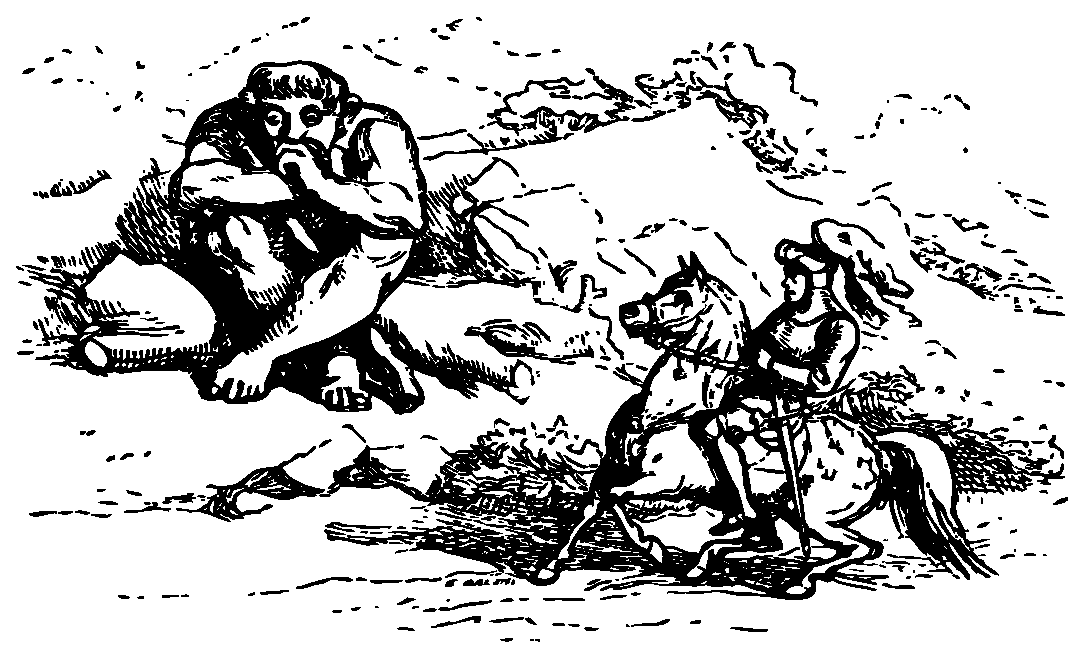
\includegraphics[scale=0.4]{../graphics/johnny_automatic_Jack_and_the_giant.eps}
\end{center}

\lettrine{D}{esde la Revolución Industrial} hasta ahora, la \textit{Era de la Información} \cite{web:informationage}, la humanidad ha cambiado por completo su manera de vivir, de pensar y de actuar. Actualmente la tecnología se ha convertido en un pilar fundamental en el progreso humano. Utilizándola como herramienta hemos sido capaces de salvar vidas, de construir edificios imposibles o incluso de conectar en el momento a personas separadas por miles de kilómetros de distancia. Y no sólo eso, en la actualidad, la manera que tenemos de consumir la información ha cambiado notablemente en los últimos 20 años. Que estamos inmersos en un mundo lleno de datos, de posibilidades, de constantes decisiones\ldots{} no es un hecho, es una realidad.

Se podría decir que el punto de inflexión lo marca la creación de Internet y su posterior expansión al público en general. Hoy en día con un móvil en nuestra mano accedemos a Google \cite{web:google}, consultamos el correo electrónico y estamos en contacto con nuestros seres queridos. Hemos sido testigos de como cada sector de la sociedad ha ido sucumbiendo, en mayor o menor medida, a las \q{maravillas} del progreso tecnológico. Algunos, en cambio, como es el sector educativo todavía se encuentran en fases tempranas de adaptación. Pero, lo que no es discutible es que existen diversos esfuerzos que tratan de crear lo que se podría denominar como \textit{Educación 2.0} \cite{web:educacion20}.

En el mercado actual existen aplicaciones o plataformas que se dedican a la educación a distancia (conocido también como \textit{e-learning} \cite{web:elearning}) para intentar llevar los procesos de enseñanza y aprendizaje a un nuevo nivel. Las ventajas que presentan esta forma de instruir son múltiples ya que eliminan ciertos factores intrínsecos a la educación tradicional como, por ejemplo, las barreras que suponen el espacio o el tiempo. Así mismo añaden mejoras en la forma de asimilar nuevos contenidos puesto que la información fluye de manera asíncrona, es decir, no hace falta tener un diálogo en directo entre la persona que imparte una materia y la que la recibe.

Otros proyectos, como puede ser \alma{} y que es el que tratamos en este escrito, surgen más bien como una necesidad de \textit{complementar} a la educación tradicional sin pretender, de ninguna manera, sustituirla por completo.

Por lo tanto, a lo largo de este proyecto se buscarán las fórmulas adecuadas para poder llevar a cabo con éxito los ideales de \alma{} que no son, ni más ni menos, que facilitar las tareas de gestión y administración utilizando para ello los \profiles{} \cite{web:explicacion-profiles} (que es una herramienta incluida dentro de la plataforma que hemos elegido y adaptado a nuestras necesidades: \tiki{} \cite{web:tikiwiki}).

\section{Objetivos del proyecto}

El objetivo fundamental de este proyecto titulado \q{\work{Gestión dinámica de grupos en una plataforma virtual basada en \tiki{}}} es doble: por una parte trata de \textit{explicar} de manera \textit{clara} y \textit{concisa} el funcionamiento de los \profiles{}. Al finalizar la lectura de este \pfc{} el lector debería ser capaz de poder crear nuevos \profiles{} que le permitan administrar la plataforma \alma{} (o cualquier otra basada en \tiki{}), así como la comprensión del funcionamiento interno de dicha herramienta de automatización. Por otra parte, se desarrollan (y se explican) unos \profiles{} preparados por el autor del escrito que atienden a las necesidades concretas de \alma{}.

En la \figureref{flujo_trabajo} se muestra el flujo de trabajo utilizado en el desarrollo de este \pfc{}:

\begin{figure}[htp]
\centering
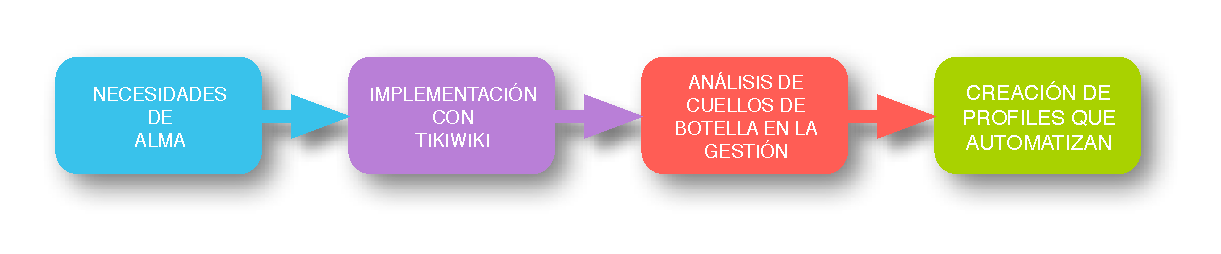
\includegraphics[width=\linewidth]{../graphics/flujo_del_pfc.eps}
\caption{Fases principales del proyecto.}\label{fig:flujo_trabajo}
\end{figure}

\section{Organización del documento}
\label{section:organizacion-documento}

Este \pfc{} está dividido en tres partes:

\begin{enumerate}
\item La primera titulada \work{Entendiendo ALMA y TikiWiki} tratará de explicar de manera detallada qué es el proyecto \alma{}, sus motivaciones, sus implicaciones, los casos de uso\ldots{} (\chapterref{estado-cuestion}), posteriormente se analizarán las diversas opciones para implementar de manera tangible y real el proyecto utilizando herramientas de \textit{software} libre: \tiki{} en nuestro caso (\chapterref{eleccion-software-wiki}).
En el \chapterref{conceptos-fundamentales-tiki} se profundizará con mayor detalle en los conceptos fundamentales de \tiki{} necesarios para entender el funcionamiento de los \profiles{} (se darán explicaciones concretas a características tan importantes como la gestión de grupos y de permisos, administración de recursos y el concepto de perspectivas).

\item La segunda parte titulada \work{Automatización de recursos con \profiles{}} se sumerge en la búsqueda soluciones concretas para atacar diversos problemas que aparecen con la gestión de una gran comunidad de usuarios.
Se explicará qué son y cómo funcionan los \profiles{} (\chapterref{profiles}). Una vez comprendido su funcionamiento interno podremos entender con detalle los \profiles{} que se han desarrollado para la gestión de \alma{} (\chapterref{gestion-dinamica}).
\end{enumerate}

Se concluye el proyecto con la última parte, \work{Sumario}, en el \chapterref{conclusiones} con las lecciones que se han aprendido a lo largo de todo el desarrollo, una autocrítica de las partes del proyecto susceptibles de mejora y se mostrarán unas ideas de lo que podrían ser las futuras líneas de trabajo. Además, al final del libro, se encuentran disponibles una serie de apéndices que sirven como complemento a la información presentada en el resto del documento. 

    
    \part{Entendiendo ALMA y TikiWiki}
      \chapter{Estado de la cuestión}
\label{chapter:estado-cuestion}

\begin{center}
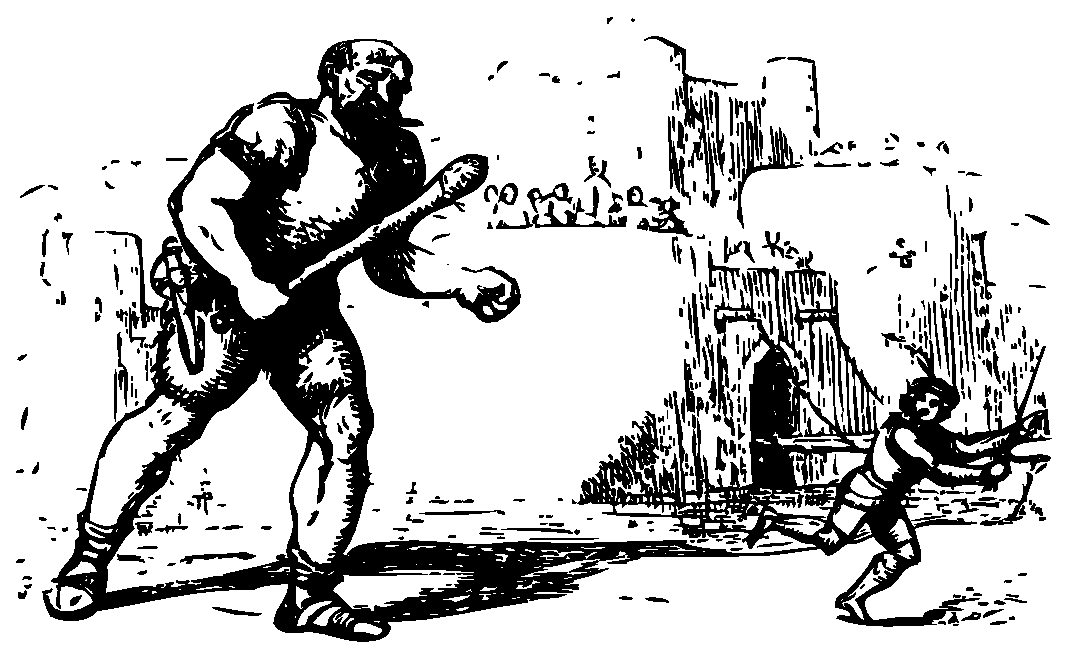
\includegraphics[scale=0.4]{../graphics/johnny_automatic_Giant_chases_Jack.eps}
\end{center}

\lettrine{E}{ste capítulo} tratará de explicar qué es el proyecto \alma{} y cuáles son sus motivaciones principales. De esta manera podemos hacernos una idea aproximada de las necesidades a cumplimentar y en qué áreas dirigir los esfuerzos. Sobre los pilares de conocimiento que se construyan aquí surgirán los demás capítulos que tratarán de dar forma a las ideas expuestas.

\section{¿Qué es el proyecto ALMA?}

En la introducción de este \pfc{} en el capítulo anterior \sectionref{introduccion} se ha comentado que uno de los sectores que todavía está en plena fase de adaptación a las nuevas tecnologías es el sector educativo. Eduardo Punset en su libro \work{Excusas para no pensar} señala que en la actualidad hay una crisis educativa y que hay que cambiar, de alguna forma, el modelo vigente \cite[No todos los niños son iguales, pág.~50]{libro:excusas-para-no-pensar}:

\begin{quotation}
\small{Curtis W. Johnson, presidente de Citistates Group y socio director de Education Evolving [\ldots], me contó que uno de los grandes errores de este sistema educativo imperante es que \guillemotleft tratamos a los niños como si fueran iguales. Los educamos igual a todos, les presentamos el material del mismo modo, y esperamos que todos aprendan las mismas cosas de la misma manera, durante el mismo día y al mismo tiempo. Esta postura no es realista, puesto que no contempla lo diferente que son los niños en muchísimas cosas, por ejemplo en el estilo de aprendizaje, pero también en el ritmo de adquisición de los conocimientos.\guillemotright{} Johnson reivindica, además, la necesidad de enseñar nuevas competencias y habilidades para que los niños y las niñas de hoy en día dominen estas técnicas para conseguir trabajo en el mundo actual. \guillemotleft La mayoría de los niños, igual que la mayoría de los jóvenes, deberán adquirir destrezas que las generaciones anteriores no tenían. Me refiero a que no solamente tendrán que aprender asignaturas básicas, sino que deberán saber cómo encontrar las cosas que necesitan saber, y luego tendrán que aprender a trabajar tal como trabaja el mundo hoy, que es principalmente en equipo [\ldots] deberán practicar el arte de la colaboración, que me parece que es el reto de colaborar con desconocidos. A todos nos encanta la idea de colaborar con nuestros amigos, y lo hacemos de muchas maneras todo el rato, pero el mundo laboral nos fuerza a llevarnos bien productivamente y crear algo de valor con gente que quizá ni siquiera nos gusta, lo cual requiere un tipo completamente distinto de educación.\guillemotright{}}
\end{quotation}

Del fragmento anterior podemos extraer las siguientes conclusiones: por un lado necesitamos hacer que la educación sea completamente personalizada, donde se adapte a las necesidades de cada persona; por otro, necesitamos centrar los esfuerzos en buscar un modelo cooperativo en los que puedan surgir las bases del aprendizaje social que es la clave que sustenta la reivindicación propuesta por Eduardo Punset y Curtis W. Johnson. Pero\ldots{} ¿qué entendemos nosotros por aprendizaje social?, ¿cómo y cuándo se produce? Esto queda explicado de manera desarrollada en \cite[pág.~1]{paper:aprendizaje-social}:

\begin{quotation}
\small{Las aulas no son los únicos entornos donde los seres humanos aprendemos, somos capaces de hacerlo en otros muchos contextos. Pensemos en cualquier escena de la vida cotidiana. Si lo hacemos descubriremos entornos no formales de desarrollo, de aprendizaje, que a menudo resultan desapercibidos. Una vez recuperada esta perspectiva de los procesos de enseñanza y aprendizaje, podemos plantearnos qué significa esta dimensión. 

Por aprendizaje social entendemos aquél aprendizaje que tiene en cuenta las interacciones sociales, es, por tanto, la forma en que los individuos adquieren conocimientos a través de la socialización e interacción con el medio.

Las teorías del aprendizaje social tienen en cuenta las interacciones sociales, pero adoptan una perspectiva de naturaleza psicológica. Destacan las relaciones entre personas que intervienen en la imitación y el modelado, y que, en consecuencia, se centran en el estudio de procesos cognitivos por los que la observación se puede convertir en fuente de aprendizaje.}
\end{quotation}


En el fragmento de arriba se menciona que el aprendizaje social \textit{requiere} de las interacciones sociales \textit{a través} de un medio en el cual los participantes pueden aprender \textit{observando}. Es innegable que una buena parte del aprendizaje, del desarrollo y de la creación de nuevas conductas en una persona tiene que ver con los factores sociales de su entorno y, no sólo eso, sino de las consecuencias positivas que le conlleva el realizar un acto que está bien visto ---bien sea por la sociedad o por los semejantes--- y que le es provechoso. Es probable que una persona que esté aprendiendo decida imitar y tomar como modelo las conductas que sean buenas ---las que se \q{premian}--- y que tienda a rechazar las que no lo son ---las que se \q{castigan}--- \cite{web:social-learning}.

Las interacciones sociales se manifiestan de múltiples maneras y formas, puesto que muchas veces su frontera no está claramente diferenciada. Podemos decir de manera análoga lo mismo para el medio. Por ejemplo, en una conversación donde intervienen dos personas, un interlocutor y un oyente (y donde es frecuente el intercambio de roles), puede ser un buen ejemplo de interacción social. El medio en este caso podría ser la voz de los participantes.
Otro ejemplo podría ser las comunicaciones indirectas en los que los individuos no interactúan en persona (\textit{chat}, teléfono, correo electrónico\ldots) y en los que el medio cobra mayor importancia, pues, condiciona la manera de recibir el mensaje. Lo que es común a ambos ejemplos es que, independientemente del medio, puede suceder que se den los mecanismos adecuados para que los individuos se enriquezcan con las aportaciones realizadas por cada participante en la conversación. Y es ahí, por lo tanto, donde se gestan las bases del aprendizaje social mencionado en el fragmento de arriba.

En la actualidad las nuevas tecnologías han creado y/o expandido nuevas formas de comunicación añadiendo o mejorando los medios existentes para expresar un mensaje. Esta última década ha supuesto un gran avance en la manera que tenemos de consumir y procesar la información. La revolución de la llamada \textit{Web 2.0} \cite{paper:innovamos} ha traído consigo una nueva forma de entender las relaciones humanas. Actualmente propuestas tan conocidas como pueden ser \textit{Flickr} \cite{web:flickr} ---donde los usuarios comparten sus fotos y votan las de los demás---, \textit{Twitter} \cite{web:twitter} ---donde los usuarios escriben en 140 caracteres lo que piensan--- o \textit{Facebook} \cite{web:facebook} ---donde el usuario tiene la posibilidad de crear un espacio virtual y tener a sus amigos cercanos en contacto--- no hacen más que reforzar el hecho de que lo social está en auge. Todos estos servicios web tienen en común la pretensión de que el usuario participe con sus semejantes de una manera cooperativa para la construcción de un conocimiento más amplio y enriquecedor.

Cabe entonces preguntarnos: ¿podemos de alguna manera aprovecharnos de las nuevas formas de interacción social y tratar de aplicarlas a un entorno de enseñanza y aprendizaje que pueda ser cooperativo? La respuesta es que si y es en esta linea en la que trabaja el proyecto \alma{}. 

La misión principal de éste es que trata de crear espacios alternativos de enseñanza y aprendizaje a los que tenemos en la actualidad sin tratar de sustituirlos  ---por ejemplo, un aula tradicional donde se imparte una asignatura--- si no más bien de complementarlos. Para ello se apoya en herramientas sociales cooperativas como son las \textit{wikis}. De esta manera se logra personalizar la educación, adaptarla al ritmo de cada individuo (como señalaban Punset y Johnson anteriormente) y hacerla más social e interactiva. En el siguiente fragmento se explica de manera detallada las ventajas que aportan usar un \textit{software wiki} en un aula \cite[pág.~4]{paper:innovamos}:

\begin{quotation}
\small{¿Qué es una \textit{wiki}? Imaginemos un sitio web cooperativo donde los usuarios pudieran crear, editar, borrar o modificar el contenido. ¡Eso es una \textit{wiki}! La \textit{wiki} más conocida es la Wikipedia \cite{web:wikipedia}, una enciclopedia creada a partir de las aportaciones de todos los usuarios que la visitan.

¿Cómo podemos utilizar una \textit{wiki} en nuestras clases? Una \textit{wiki} nos permite crear un espacio de trabajo cooperativo con nuestros alumnos. Podemos montar una \textit{wiki} para editar, entre todos, los apuntes de una asignatura (\textit{wiki-apuntes}), o podemos utilizarla para crear un glosario con los términos conceptuales que surjan durante las clases. Incluso podemos proponer a los alumnos que mejoren algún artículo ya existente en la Wikipedia y que guarde relación con su asignatura, como por ejemplo este: \url{http://es.wikipedia.org/wiki/Derecho_romano}.

Son muchas las posibilidades de trabajo que acerca un espacio \textit{wiki} al proceso de enseñanza y aprendizaje de los alumnos, y como docentes debemos indagar en ellas.

Todas las ediciones y cambios que se hacen en una \textit{wiki} quedan registradas, de forma que el profesor sabe qué ha editado quien, y cuando lo ha hecho. Una \textit{wiki} permite a los alumnos y al profesor editar de una forma muy sencilla los contenidos de un sitio web. Todos pueden trabajar editando un glosario con los conceptos de la asignatura, y además establecer discusiones sobre cada concepto en el que trabaja la clase. Es por lo tanto una herramienta sencilla y que facilita enormemente la tarea de editar contenidos en grupo.

Sobre la utilización de las \textit{wikis} en la docencia podemos decir muchas más cosas. Rompen la asimetría y la unidireccionalidad de la enseñanza, de modo que los propios alumnos son los que enseñan a sus compañeros, pues el conocimiento se construye entre todos. El profesor adquiere nuevos roles: facilitador, moderador, orientador, y evaluador (continuo). También lo hacen los alumnos: colaboradores, cooperadores y capaces de enseñar a sus compañeros. Las barreras de la clase se superan de tal forma que podemos compartir y generar conocimiento con el resto del mundo.}
\end{quotation}

Como queda demostrado arriba las \textit{wikis}, por su naturaleza, se asientan en los principios de las \textit{interacciones sociales}, es decir, se nutren de las participaciones de todas las personas. Además, su máximo interés reside en el hecho de que se dispone de una total libertad para poder modificar tantas veces se quiera el \textit{mensaje} (pudiendo crear nuevos contenidos, editarlos, borrarlos y recuperarlos cuando y como deseemos). A esto es a lo que se conoce como \textit{filosofía wiki} (\figureref{filosofia_wiki}) \cite{video:wikis-plain-english}. Lo maravilloso de esta forma de trabajar es que, de manera inconsciente, se acaba creando lo que \citeauthor{libro:comunidades-de-practica-wenger-primera-edicion} en su libro \work{Communities of Practice: Learning, Meaning, and Identity} \cite{libro:comunidades-de-practica-wenger-primera-edicion} denominó por primera vez, en \citeyear{libro:comunidades-de-practica-wenger-primera-edicion}, como \textit{comunidades de práctica}. Y\ldots{} ¿qué son exactamente?

\begin{figure}
\centering
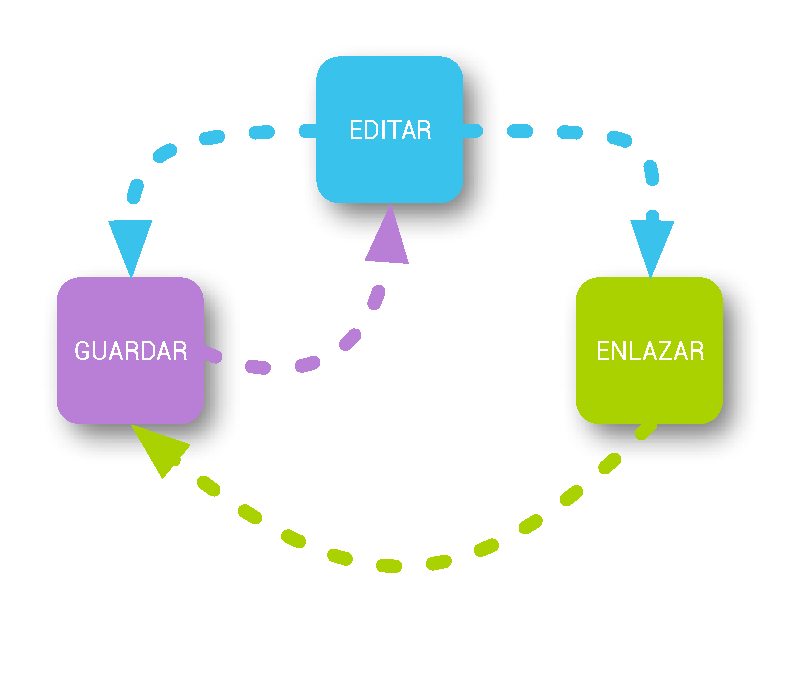
\includegraphics[width=\linewidth]{../graphics/fig_filosofia_wiki.eps}
\caption{Flujo de trabajo en la filosofía \textit{wiki}. Como podemos observar, éste se repite indefinidamente.}\label{fig:filosofia_wiki}
\end{figure}
 
Una definición, más o menos formal, podría decir que: \q{las comunidades de práctica se originan cuando existe un grupo de individuos que comparten un interés, o un conjunto de problemas o una pasión sobre un tema determinado y, que profundizan tanto su conocimiento y experiencia en el área, que lo que produce es que las relaciones entre los distintos miembros se acaban fortaleciendo} \cite{paper:filwit}.

Las comunidades de práctica se pueden dar en múltiples ámbitos (o en todos a la vez), es más, es bastante probable que cualquier persona que tenga una afición, sea cual sea, por el mero hecho de compartir sus gustos con otras personas ésta pertenezca ya, sin saberlo, a una comunidad de práctica. Aunque hay que discernir que no todas las comunidades a las que se puede pertenecer son comunidades de práctica. Para que lo sean se deben dar tres características fundamentales:

\begin{itemize}
\item \textit{Dominio}: es el campo de interés compartido por la comunidad y es el que crea una identidad común al grupo.

\item \textit{Comunidad}: es aquí donde los miembros establecen las relaciones que les permiten aprender y, a su vez, exponer su experiencia y su conocimiento en un tema determinado.

\item \textit{Práctica}: los miembros forman parte del proceso mismo, participando en actividades de manera conjunta y donde se comparten los intereses de la comunidad.
\end{itemize}

Como las comunidades de práctica se pueden dar en cualquier lugar es por eso que se mencionaba anteriormente que el \textit{software wiki} las genera de manera inconsciente. Si lo pensamos bien, podemos llegar a la siguiente conclusión: el \textit{software wiki} es utilizado de tal manera que es un \textit{medio} que sirve como causa para lograr un \textit{fin} que no es otro que el \textit{dominio}, la \textit{comunidad} y la \textit{práctica}. (En la \figureref{comunidades_de_practica} podemos ver a diferentes comunidades de práctica trabajando en grupos y que están implementadas sobre una plataforma \textit{wiki} cualquiera.)

\begin{figure}
\centering
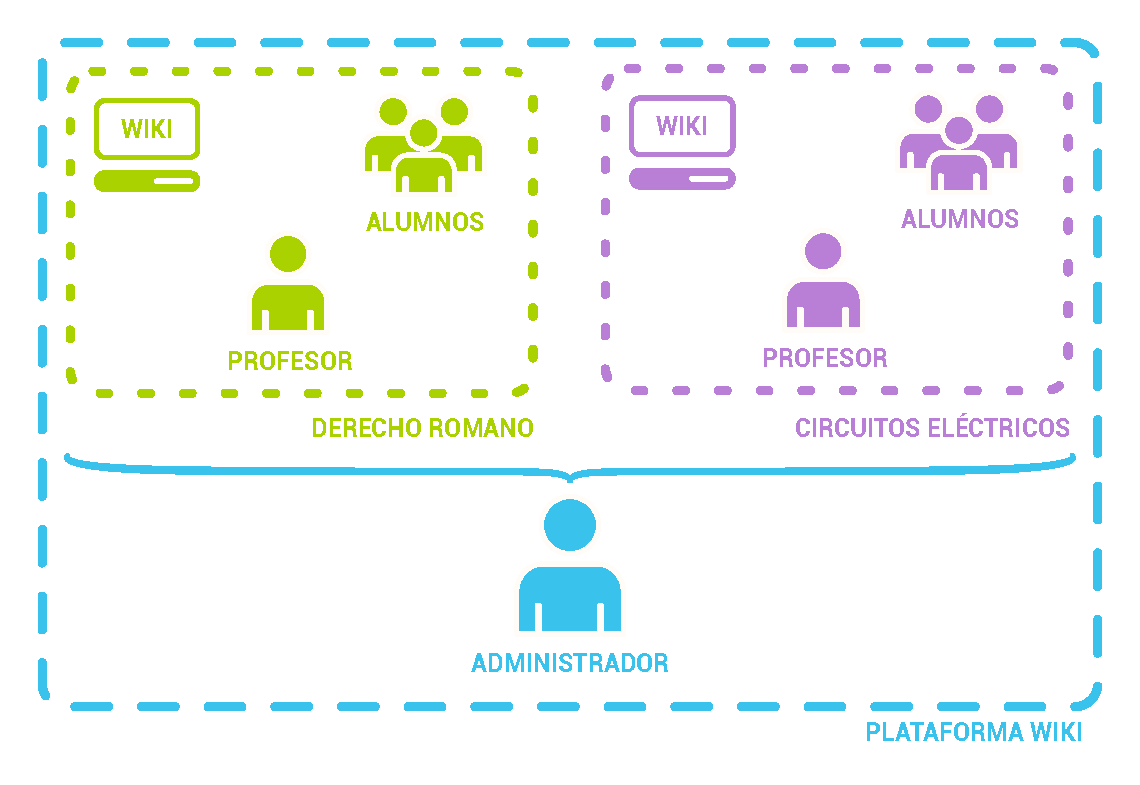
\includegraphics[width=\linewidth]{../graphics/fig_comunidades_de_practica.eps}
\caption{Distintas comunidades de práctica trabajando conjuntamente en su propio dominio. El administrador de la plataforma es el encargado de que todo funcione correctamente.}\label{fig:comunidades_de_practica}
\end{figure}

Otro aspecto importante que hay que tener en cuenta y que se puede ver analizando la \figureref{comunidades_de_practica}, son los roles y las interacciones que se producen en una comunidad de práctica. \citeauthor{libro:comunidades-de-practica-wenger} en el libro \work{Cultivating Communities of Practice: A Guide to Managing Knowledge} \cite{libro:comunidades-de-practica-wenger} sostienen que no sólo es significativo pensar en las tres características que conforman las comunidades de práctica, sino que hay que dar un paso adelante y analizar los diferentes perfiles que hay dentro de ellas. Esto se debe a que no todos los miembros de una comunidad de práctica participan en ésta de forma equitativa; cada persona tiene un nivel distinto de interés en el papel que le toca desempeñar. Estos son los diferentes roles o niveles de participación que podemos encontrar (clasificados de menor a mayor grado de implicación):

\begin{itemize}

\item \textit{Agentes externos}: No pertenecen directamente a la comunidad pero muestran una inclinación en ésta, puede ser que como clientes o porque comparten algún punto de interés.

\item \textit{Miembros periféricos}: Este grupo pertenece a la comunidad y su característica principal es que participan en escasas ocasiones y son el grupo mayoritario. Normalmente suelen observar las interacciones de los miembros activos, del núcleo y de los coordinadores. Las motivaciones del porqué no participan suelen ser porque consideran que sus aportaciones no son importantes para la comunidad o que no poseen con la autoridad suficiente para que sean tenidos en cuenta. Otros, en cambio, consideran simplemente que no quieren participar porque no disponen de tiempo suficiente para ser más activos. Aún así, sus actividades periféricas, son sumamente importantes para el resto ya que gracias a su observación de todo lo que sucede dentro, consiguen obtener una visión amplia de todo lo que se expone.

\item \textit{Miembros activos}: Este grupo son aquellos que, según Wenger y col., suelen participar ocasionalmente en los foros u otras actividades de la comunidad pero sin llegar al nivel de intensidad de los miembros del núcleo. No suele ser un grupo muy amplio, ya que quizá no llegue a más del 15 ó 20\% de la comunidad.

\item \textit{Núcleo}: Es, por lo general, el grupo más compacto y pequeño que participa activamente en todas las actividades de la comunidad de una forma activa. Son los que guían a la comunidad a través de una agenda de actividades. Conforme la comunidad va madurando, este grupo suele tomar una buena parte del liderazgo junto con el coordinador. Es un grupo minoritario que no comprende más del 10\% de los participantes.

\item \textit{Coordinador}: Es el encargado de organizar eventos y conectar a los diferentes miembros de la comunidad. Su contribución se basa en que la comunidad esté enfocada en su dominio, que mantenga relaciones entre sus miembros y otras comunidades, y que desarrolle su práctica. La dedicación de esta persona como coordinador es bastante alta, típicamente los valores oscilan entre 20 y el 50\% de su tiempo. Además, sus otras funciones principales son:
\begin{itemize}
\item Vela por que la comunidad esté siempre activa y que se produzcan contribuciones de ésta a los demás miembros.
\item Relaciona informalmente miembros de la comunidad.
\item Planea y facilita eventos en la comunidad.
\item Contribuye en la construcción de la práctica. Esto incluye trabajar en la administración del conocimiento en la comunidad, lecciones aprendidas, mejores prácticas y métodos para el aprendizaje.
\item Identifica cuestiones o temas importantes en el dominio de la comunidad.
\item Posee una buena relación con el Núcleo y distribuye ciertas tareas con dicho grupo.
\end{itemize}
\end{itemize}

Saber identificar estos roles nos ayuda a entender como funcionan las comunidades de práctica internamente. También nos da una idea general de que características necesita una plataforma \textit{wiki} para que la implementación sea lo más afín a la definición dada.

Por lo tanto, en el siguiente capítulo nos veremos en la necesidad de buscar un \textit{software} que pueda implementar de manera fiable todo lo que aquí se ha explicado ya que la clave que sustenta al proyecto \alma{}, son al fin y al cabo, las comunidades de práctica.
      \chapter{Elección de un software wiki}
\label{chapter:eleccion-software-wiki}

\begin{center}

\includegraphics[scale=0.4]{../graphics/johnny_automatic_giant_going_to_castle.eps}
\end{center}

\lettrine{E}{n este capítulo} se analizarán las necesidades que tiene el proyecto \alma{} y se explicarán las causas del porqué de la elección de \tiki{} como herramienta principal frente a otras alternativas similares. Para finalizar se dará una visión genérica a las características más importantes de dicho \textit{software} y se informará al lector de los enlaces de interés para expandir su conocimiento sobre la plataforma.

\section{¿Qué necesidades tiene ALMA?}

A lo largo de todo el capítulo anterior se han ido razonando las motivaciones que tiene \alma{} siguiendo el modelo de las comunidades de práctica. Intuitivamente sabemos que la índole de este proyecto queda englobada en un entorno educativo que involucra grupos de usuarios trabajando alrededor de una temática concreta. Por lo tanto, es lógico pensar qué tipo de herramienta vamos a utilizar para implementar el concepto y para ello nos debemos preguntar por las necesidades concretas que debe responder el \textit{software}. A continuación, se listan los requisitos más importantes que consideramos a tener en cuenta:

\begin{itemize}
\item \textit{Wikis}: Dado que este es el pilar fundamental en el que se basan las comunidades de práctica, necesitamos que el \textit{software} que elijamos posea una implementación robusta de la filosofía \textit{wiki}. 

\item \textit{Gestión excelente de grupos y permisos asociados a ellos}: Una implementación correcta en la gestión de los grupos y sus permisos nos permite dividir las comunidades de práctica en distintos ámbitos (quizá no interese que los alumnos que pertenecen a una asignatura de \q{Circuitos Eléctricos} se mezclen con los alumnos que pertenecen a la asignatura de \q{Estadística}, ni que tampoco puedan modificar los elementos sobre los que estén trabajando estos últimos).

\item \textit{Facilidad en la instalación, mantenimiento y manejo}: Buscamos que nuestro \textit{software} no posea ninguna complejidad a la hora de instalarlo, que use componentes robustos y que, en general, el manejo sea sencillo (que no tiene porqué significar necesariamente que sea simple).

\item \textit{Automatización}: Es probable que si la plataforma es usada por mucha gente dicha gestión, por parte de un administrador, deje de ser algo trivial (asignación de permisos, creación de nuevas comunidades de práctica, establecer usuarios a diferentes grupos\ldots).

\item \textit{Robustez}: ¿Podemos estar seguros de que la plataforma soportará una gran cantidad de usuarios?

\item \textit{Que sea adaptable}: El \textit{software} debe permitir crear cualquier estructura posible. En nuestro caso el concepto de las comunidades de práctica como se mostró en la \figureref{comunidades_de_practica} en el \chapterref{estado-cuestion}.
\end{itemize}

\section{¿Qué herramientas existen?}

En el mercado actualmente podemos encontrar muchas propuestas que nos permiten implementar de múltiples maneras y formas un sistema de aprendizaje virtual (\textit{e-learning}). La denominación que reciben este tipo de \textit{software} es: \lms{}. Y es un \textit{software} que se instala en un servidor web y que se emplea para administrar, distribuir y controlar las actividades de formación no presencial de una institución o organización \cite{web:lms}.

Las principales funciones del \lms{} son: gestionar usuarios, recursos, así como materiales y actividades de formación. También se encargan de administrar el acceso al mismo, controlar y hacer seguimiento de los procesos de aprendizaje, realizar evaluaciones, generar informes, gestionar servicios de comunicación como foros de discusión\ldots{} En cambio, generalmente, no incluyen posibilidades de autoría, es decir, que se pueda crear contenidos propios, sino que se centra en gestionar contenidos creados por fuentes diferentes.

\alma{}, \textit{per se}, no utiliza todas las características a las que se adscriben los \lms{}. Por ejemplo, el hecho de que no suelen incluir contenidos generados por los propios usuarios es algo que contradice expresamente la naturaleza de este proyecto. Este pequeño detalle, como veremos más adelante, nos hizo descartar algunas propuestas por no cumplir con los requisitos necesarios.

Por lo tanto, si \alma{} no se puede categorizar dentro de un \lms{} propiamente dicho (aún compartiendo muchas de sus ideas), ¿qué es entonces? Podríamos responder que es un híbrido entre un \lms{} y un \cms{} \cite{web:cms}.

Un \cms{} es un programa que, al igual que un \lms{}, se puede instalar en un servidor web y permite, de manera sencilla, la creación y la administración de contenidos (principalmente para ser consumidos en páginas web) por parte de los administradores, editores, participantes y demás roles.

En \alma{} los contenidos son creados por los propios usuarios, otras veces, por alguien externo. Por lo tanto, ¿qué propuestas encontramos en el mercado que más o menos se ajusten a un híbrido de un \lms{} y un \cms{}? Se listan a continuación las opciones más relevantes:

\begin{itemize}
\item WebCT o BlackBoard
\item Moodle
\item MediaWiki
\item \tiki{}
\end{itemize}

WebCT, conocido también como BlackBoard \cite{web:blackboard}, es, por definición expresa, el sistema que ha determinado, tal y como lo conocemos, las bases de los \lms{} de manera concreta y del aprendizaje virtual (\textit{e-learning}) en general. Nuestra universidad lo usa en múltiples cursos y asignaturas de las diferentes carreras que se imparten \cite{web:webct-uah}.

No negamos que se trata de un \textit{software} que es bastante competente en su terreno, pero la mayor desventaja que tiene es que su licencia es privativa y por ello el usuario no tiene ningún derecho a poder copiar, estudiar, modificar y redistribuir el código de la plataforma \cite[pág~2]{paper:innovamos}. Es más, tendríamos que pagar una licencia por el uso de la misma. Por lo tanto desde el principio consideramos que no era una opción plausible. 

La alternativa más conocida a WebCT es Moodle \cite{web:moodle}. Posee muchas de las características del primero más algunas suyas propias. Nuestra universidad también lo usa en determinadas asignaturas \cite{web:moodle-uah}. Sin embargo, tampoco es una opción a tener en cuenta porque principalmente está centrado en distribuir cursos (o lecciones) provenientes de una fuente central (el profesor por ejemplo) y unos alumnos trabajando sobre esos materiales. Realmente se pueden ver como una ayuda a la clase, o como una forma de sustituirla, pero no para complementarla de manera creativa a como lo propone el concepto de las comunidades de práctica. Por lo que también quedó descartada.

MediaWiki \cite{web:mediawiki} es quizá la más conocida de las expuestas, puede que no de manera directa, pero es el \textit{software} que corre la Wikipedia \cite{web:wikipedia}.
Como su propio nombre indica se centra en las \textit{wikis} de manera exclusiva (lo cual es bastante positivo porque es uno de los requisitos que pedimos para \alma{}). Otro aspecto es que se puede instalar muy fácilmente en cualquier servidor que cumpla unos requisitos mínimos. Además posee una comunidad de usuarios bastante amplia y hay muchos manuales que explican como configurar y modificar el propio \textit{software}. Sin embargo, como características negativas es que la gestión y la administración de los usuarios no es tan trivial, tampoco se pueden crear grupos aislados de usuarios ni controlar los accesos a las diferentes páginas \textit{wikis} de una manera selectiva, y no hay posibilidad de automatizar ciertas tareas de gestión rutinarias. Por lo tanto es otra opción que descartamos.

\section{¿Por qué se escogió TikiWiki?}

\begin{figure}
\centering

\includegraphics[scale=0.75]{../graphics/tiki-logo.png}
\caption{Logotipo de Tikiwiki.}\label{fig:tikiwiki_logo}
\end{figure}

De las cuatro opciones que se han presentado, la última que queda es \tiki{}. Fue escogida por los siguientes motivos (responde a muchas de las peticiones que pusimos antes y añade más características que no habíamos pensado pero que, sin embargo, nos son útiles):

\begin{itemize}
\item \textit{Versátil}: El diseño de \tiki{} es lo que se conoce como un \q{todo-en-uno}, es decir, aglutina muchas características en un sólo \textit{software}. Esto es positivo porque actualmente \alma{} utiliza las \textit{wikis} como medio para crear las comunidades de práctica, pero, en algún futuro se podrían utilizar otras herramientas que sirviesen para el mismo propósito, por ejemplo, foros de discusión. Al tener \tiki{} integradas las \textit{wikis}, los foros, los \textit{blogs}, galerías de imágenes, mapas\ldots{} dentro del propio \textit{software}, nos olvidamos de tener que instalar complementos (\textit{plug-ins}) u otras herramientas externas para conseguir el mismo efecto.

\item \textit{Fiable}: Muchos proyectos de código abierto (y otros tantos comerciales) utilizan \tiki{} como motor principal para gestionar sus \textit{wikis} (y otras necesidades). Como ejemplo importante que utilice \tiki{} encontramos al motor de 3\textsc{d} Ogre \cite{web:ogre-tikiwiki, web:tikiwikis-destacadas}.

\item \textit{Flexible}: \tiki{} se puede adaptar a cualquier necesidad ya que, al incorporar una gran cantidad de opciones, puede ser utilizado como una \textit{wiki}, como un \textit{blog} para una persona, un gestor de errores en programación (\textit{bug tracker}),  una comunidad de usuarios, un portal de noticias, una web corporativa \cite{web:tiki-use-cases}\ldots{} La imaginación es nuestro límite.

\item \textit{Profiles}: Como apoyo al punto anterior, y debido a que \tiki{} posee más de 1500 opciones de configuración distintas, surgieron los \profiles{}. Éstos permiten modificar cualquier opción posible de la plataforma de \tiki{} de una manera sencilla y eficaz utilizando ficheros de \q{texto plano}. Esta fue la característica principal de la elección de \tiki{} como \textit{software} y con la que se consiguió implementar \alma{} con éxito.

\item \textit{Perspectivas}: Otra de las habilidades de este \textit{software} que destaca por si sola es que permite, por ejemplo, que para un mismo usuario la experiencia usando el \textit{software} de \tiki{} sea completamente diferente dependiendo de las acciones que realice.

\item \textit{Excelente gestión de usuarios y de permisos}: Con \tiki{} se obtiene una jerarquía de permisos muy fina y detallada, se pueden aplicar de manera global a todos los usuarios, o pueden ser concretos tanto a un usuario como a un grupo o bien a un recurso (una \textit{wiki}) permitiendo dar acceso o denegarlo acorde a las necesidades que se tengan.

\item \textit{Facilidad de instalación}: Para funcionar \tiki{} sólo necesita un servidor capaz de ejecutar código en \php{} 5 \cite{web:php} y una base de datos \textsc{m}y\textsc{sql} \cite{web:mysql} para guardar la información.

\end{itemize}

\subsection{Información de interés sobre TikiWiki}

A continuación dejamos al lector interesado en obtener más información una serie de enlaces importantes sobre \tiki{} y que varían desde la descarga de el propio \textit{software} hasta casos complejos de configuración, a saber:

\begin{itemize}
\item Información básica de la plataforma (\url{http://tiki.org}): Aquí podemos descargar el \textit{software} y obtener información básica de sus características principales. Es útil para averiguar si \tiki{} se ajusta a nuestras necesidades o no.

 \item Documentación genérica (\url{http://doc.tiki.org}): Esta página está orientada a la obtención de información por parte del administrador de la plataforma. Cualquier necesidad que surja a la hora de configurar el \textit{software}, aquí es probable que se encuentre la respuesta.
 
 \item Desarrollo (\url{http://dev.tiki.org}): Esta \textit{wiki} está preparada para los desarrolladores del código ya que se muestran las últimas novedades que se producen en el código fuente de \tiki{}, así como también nuevas características que se añadirán a versiones futuras, implementaciones que se han realizado y en general cualquier tipo de documentación útil para la gente que quiera programar.

 \item \profiles{} (\url{http://profiles.tiki.org}): Aquí se puede encontrar toda la información importante sobre la información relacionada con la configuración, desarrollo y creación de los \profiles{}. También es un punto de intercambio de nuevos \profiles{} que hayan creado otros usuarios. Instamos al lector interesado a que visite esta página web para obtener una información más detallada sobre esta herramienta.

 \item Canal de \textsc{irc} (\url{http://webchat.freenode.net/?channels=tikiwiki}): En este canal de \textsc{irc} se alojan los principales \q{sabios de \tiki{}} que nos pueden ayudar siempre que lo necesitemos.
\end{itemize}

      \chapter{Conceptos fundamentales de TikiWiki}
\label{chapter:conceptos-fundamentales-tiki}

\begin{center}

\includegraphics[scale=0.4]{../graphics/johnny_automatic_Jack_eating_with_the_giant.eps}
\end{center}

\lettrine{E}{n los capítulos anteriores} se han descrito conceptos tan importantes como: qué es \alma{}, qué son las comunidades de práctica y, sobre todo, qué tipo de \textit{software} nos puede ayudar a conseguir nuestro objetivo. En este capítulo nos centraremos en dar una visión detallada de cómo se puede implementar una comunidad de práctica con las herramientas que tiene disponible por defecto \tiki{} (sin utilizar, todavía, ningún tipo de automatización con \profiles{}). Esto nos ayudará a, por una parte, tener una visión genérica de las capacidades que nos brinda el \textit{software} (y hasta que punto podemos \q{adaptarlo} a nuestras necesidades) y por otra, a darnos cuenta de que crear comunidades de práctica es una tarea repetitiva y tediosa para un administrador.

\section{¿De qué manera podemos implementar una comunidad de práctica con \tiki{}?}

Si recordamos, en la \figureref{comunidades_de_practica} del \chapterref{estado-cuestion} aparecían múltiples comunidades de práctica (en recuadros de color verde y lila, las asignaturas de \q{Derecho Romano} y \q{Circuitos Eléctricos}, respectivamente) dentro de una plataforma wiki que era dirigida por un administrador (el recuadro azul). A continuación, en la \figureref{comunidad_de_practica_derecho_romano}, se ha cogido del ejemplo anterior la comunidad de práctica de \q{Derecho Romano} y será sobre ella donde se ilustrarán los conceptos más importantes que debemos de conocer de \tiki{} para implementar las comunidades de práctica. Hay que añadir que toda información que se presente aquí no pretende ser exhaustiva en cuanto a demostraciones de como administrar la plataforma, ya que, no es el objetivo principal de este \pfc{} hacerlo. Si bien cuando se considere oportuno, se instará al lector a buscar más información dentro de los enlaces presentados en el capítulo anterior y de los que se presenten en éste. ¡Comenzamos!

\begin{figure}
\centering

\includegraphics[width=.8\linewidth]{../graphics/fig_comunidad_de_practica_derecho_romano.eps}
\caption{La comunidad de práctica de la asignatura de Derecho Romano.}\label{fig:comunidad_de_practica_derecho_romano}
\end{figure}

\subsection{Concepto de recursos}
\label{section:concepto-recursos}

Un \textit{recurso} no es, ni más ni menos, que cualquiera de las herramientas que nos pone \tiki{} a nuestra disposición (\textit{wikis}, foros de discusión, galerías de imágenes\ldots{}) y que puede ser utilizado por las comunidades de práctica para implementar sus actividades (\figureref{comunidad_de_practica_derecho_romano_recursos}).
La creación de recursos en \tiki{} es bastante sencillo, ya que, basta con que un administrador acuda a la página de administración de la plataforma (por defecto: \url{http://localhost/tiki-admin.php?page=features}\footnote{Asumimos que tenemos \tiki{} correctamente instalado, funcionando con una base de datos habilitada para tal efecto y en nuestro caso se está ejecutando en un ordenador local, de ahí que se use \texttt{http://localhost} como dominio principal de la dirección de ejemplo \cite{web:instalacion-tiki}.}) y habilite las características que desea. (En la \figureref{panel_habilitar_recursos_tiki} vemos como se pueden activar y desactivar los diferentes recursos que posee la plataforma.) 
 Una vez que el administrador ha habilitado los recursos que desea, puede visitar la página: \url{http://localhost/tiki-admin.php} y configurar las opciones pertinentes a dicho recurso (\figureref{panel_de_recursos}).


Cabe añadir que dichos recursos son globales, es decir, sin haber cambiado ninguna opción más de la plataforma, se crearía una sola \textit{wiki} o una sola galería de imágenes o un foro. Estos elementos serían comunes a todos los usuarios (no habría todavía ningún concepto de comunidades de práctica). 

\begin{figure}
\centering

\includegraphics[width=.8\linewidth]{../graphics/fig_comunidad_de_practica_derecho_romano_recursos.eps}
\caption{Los recursos son aquellas herramientas que \tiki{} nos pone a nuestra disposición: \textit{Wikis}, Foros, Galerías de Imágenes ...}\label{fig:comunidad_de_practica_derecho_romano_recursos}
\end{figure}

\begin{figure}
\centering
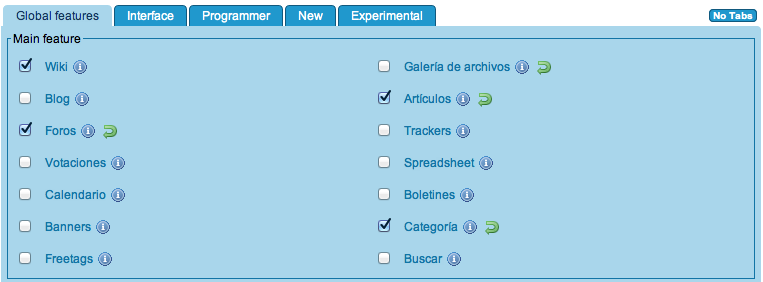
\includegraphics[width=\linewidth]{../graphics/fig_panel_habilitar_recursos_tiki.png}
\caption{Panel de habilitación de recursos en \tiki{}.}\label{fig:panel_habilitar_recursos_tiki}
\end{figure}

\begin{figure}
\centering
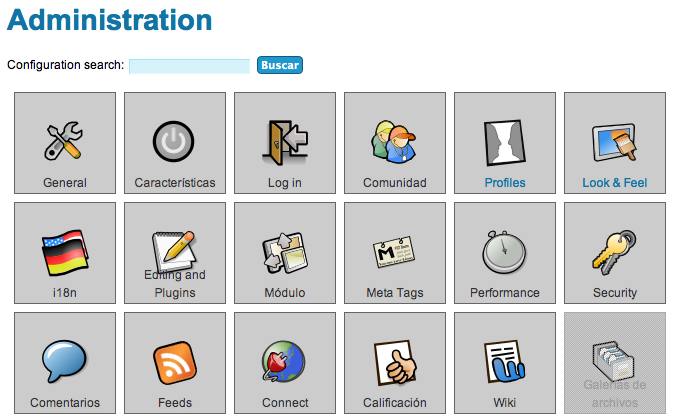
\includegraphics[width=\linewidth]{../graphics/fig_panel_de_recursos.png}
\caption{Panel de administración principal. Nos indica con transparencias si un recurso está habilitado o no (en este caso en concreto el recurso \q{galería de archivos} está desactivado). Si pinchamos en el icono del recurso nos lleva a su página de configuración.}\label{fig:panel_de_recursos}
\end{figure}

\subsection{Concepto de grupos}

\begin{figure}
\centering
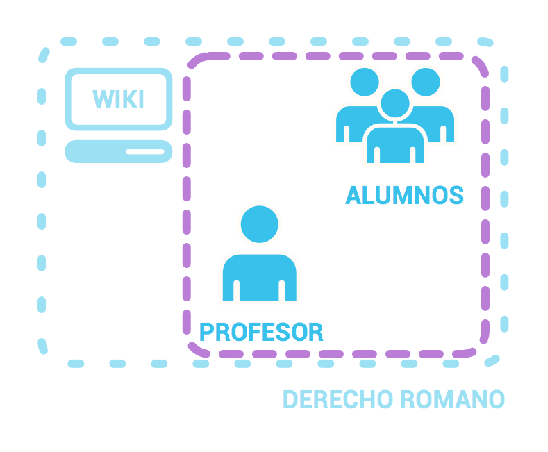
\includegraphics[width=.8\linewidth]{../graphics/fig_comunidad_de_practica_derecho_romano_grupos.eps}
\caption{Los grupos nos permiten aunar usuarios según preferencias. Pueden ser tan granulares como deseemos y un usuario puede pertenecer a uno o varios grupos.}\label{fig:comunidad_de_practica_derecho_romano_grupos}
\end{figure}

Los \textit{grupos} (como su propio nombre indica) se utilizan en \tiki{} como un contenedor donde se pueden agrupar, utilizando algún criterio de clasificación, a distintos usuarios de la plataforma. Se utilizan para múltiples propósitos pero, entre ellos, el más importante es que se les puede otorgar (o eliminar) permisos de acceso a los diferentes recursos (por ejemplo: que un determinado grupo pueda editar una página \textit{wiki} pero que a su vez no pueda subir imágenes a ésta). Esta característica nos es útil, en nuestro caso, porque podemos crear múltiples grupos que engloben a los diferentes roles que existen (profesores y alumnos) y asignarles a éstos diferentes permisos de acceso a los recursos (\figureref{comunidad_de_practica_derecho_romano_grupos} y \figureref{panel_administracion_grupos}).

\begin{figure}
\centering
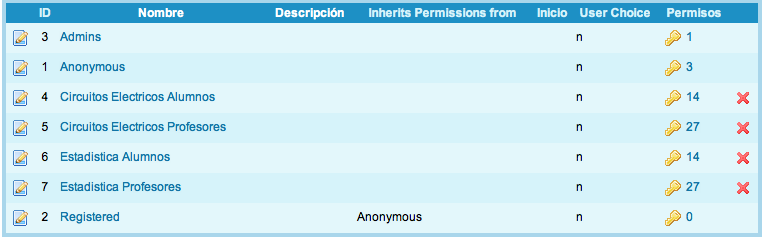
\includegraphics[width=\linewidth]{../graphics/fig_panel_administracion_grupos.png}
\caption{Panel de administración de grupos.}\label{fig:panel_administracion_grupos}
\end{figure}

Por defecto, \tiki{} genera tres grupos importantes que son tratados de manera especial por el \textit{software}: \texttt{Anonymous}, \texttt{Registered} y \texttt{Admins}. Éstos engloban a cualquier usuario de la plataforma: al primero, pertenecen todos aquellos usuarios que están visitando \tiki{} pero que no se han registrado o que no han iniciado una sesión en la plataforma; al segundo, si hacemos una traducción directa del inglés, pertenecen todos aquellos que si han iniciado una sesión en el \textit{software}; al tercero, pertenecen todos aquellos usuarios que tienen roles de administradores, es decir, los que poseen el máximo poder administrativo de la propia plataforma.  

También hay que destacar que otra de las características que poseen los grupos en \tiki{} es que se pueden crear unos dentro de otros (y montar así una jerarquía de grupos). Esto permite el que se pueda concebir un grupo cualquiera con unos permisos genéricos y luego que otros grupos hereden dichos permisos e ir restringiéndolos según se necesite. Se evita duplicar esfuerzos aunque, en nuestro caso, no utilizamos esta característica para implementar las comunidades de práctica. 

Para más información relativa a los grupos podemos visitar: \url{http://doc.tiki.org/Groups}.

\subsection{Concepto de categorías}

Al igual que con los grupos podíamos asociar a usuarios en distintos conjuntos, las \textit{categorías} es un concepto similar que funcionan de la misma manera, sólo que en lugar de agrupar usuarios permiten clasificar los recursos de \tiki{}. Cualquier recurso que existe en la plataforma es susceptible de ser categorizado incluyendo: \textit{blogs}, galerías de imágenes, artículos, encuestas, foros, páginas \textit{wiki}, galerías de archivos, etcétera. Y al igual que con los grupos, un recurso puede pertenecer a una o varias categorías y que cada categoría tenga sus propios permisos individuales (\figureref{comunidad_de_practica_categorias}).

\begin{figure}
\centering

\includegraphics[width=.8\linewidth]{../graphics/fig_comunidad_de_practica_derecho_categorias.eps}
\caption{Conjunto de recursos agrupados en una categoría y que pertenecen a la comunidad de práctica de Derecho Romano.}\label{fig:comunidad_de_practica_categorias}
\end{figure}

El principal uso que se le da a las categorías es para controlar el acceso a un conjunto específico de recursos. Al establecer permisos concretos en una categoría, lo que hace es que todos los permisos globales que tenían los recursos por si solos desaparecen y son sobreescritos por los que hay en la categoría (en la siguiente sección se verá de manera más detallada como se aplican los permisos).

Las categorías también se pueden utilizar para ayudar en la navegación del sitio o para crear un conjunto de recursos relacionados por algún criterio. Por ejemplo: en la \figureref{listado_categorias} observamos que hay una categoría llamada \q{Circuitos Eléctricos}, dentro de ella estarían los recursos que pertenecen a dicha comunidad de práctica.

\begin{figure}
\centering
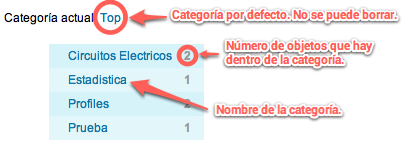
\includegraphics[scale=.8]{../graphics/fig_listado_categorias.png}
\caption{Listado de todas las categorías que se han creado en \tiki{}.}\label{fig:listado_categorias}
\end{figure}

Como sucedía con los grupos, \tiki{} crea una categoría especial denominada \texttt{Top} que es la categoría madre donde todas las demás dependerán de ella, es decir, heredarán de esa categoría. También es posible crear categorías dentro de categorías y obtener así un árbol jerárquico (aunque nosotros no exploraremos esa opción ya que no nos es necesario para poder crear las comunidades de práctica).

Las categorías en \tiki{} no vienen habilitadas por defecto, así que es tarea del administrador decidir si desea tenerlas activas o no.
Para administrarlas se debe de ir a la siguiente dirección: \url{http://localhost/tiki-browse_categories.php} y ahí nos encontraremos con el panel de la \figureref{listado_categorias}. Si se pincha en una categoría se podrá obtener información más detallada sobre ésta, los recursos que tiene asociados y los permisos que posee\ldots{} (\figureref{vista_categoria_circuitos}) 

Para averiguar más sobre las categorías podemos visitar: \url{http://doc.tiki.org/Category}.

\begin{figure}
\centering

\includegraphics[scale=.8]{../graphics/fig_vista_categoria_circuitos.png}
\caption{Vista detallada de la categoría Circuitos Eléctrico y sus recursos asociados.}\label{fig:vista_categoria_circuitos}
\end{figure}

\subsection{Concepto de permisos}
\label{section:concepto-permisos}

\begin{figure}
\centering
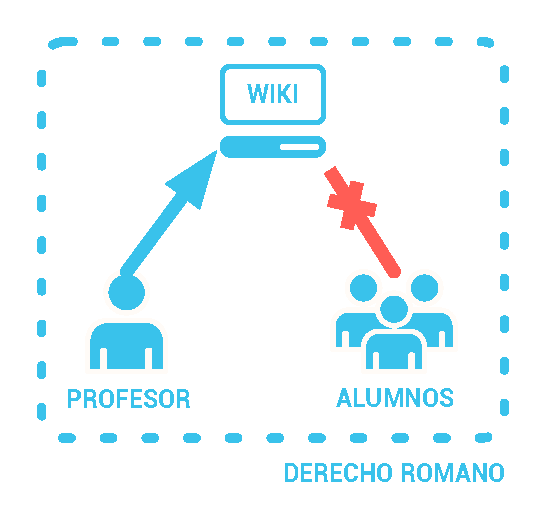
\includegraphics[width=.8\linewidth]{../graphics/fig_comunidad_de_practica_derecho_permisos.eps}
\caption{Concepto de lo que son los permisos en \tiki{}.}\label{fig:concepto_permisos}
\end{figure}

Los \textit{permisos} son una de las herramientas más poderosas que posee \tiki{} y es con ellos con los que podemos crear, junto con las perspectivas \sectionref{concepto_perspectivas}, el concepto de las comunidades de práctica. Un administrador de la plataforma puede decidir quién y bajo qué circunstancias un usuario o un grupo puede acceder a un recurso y modificarlo. El esquema de permisos de \tiki{}, sobre todo al principio, puede parecer un poco caótico (en parte debido a como se ha implementado el panel de administración), pero, una vez acostumbrados podemos personalizar la plataforma a nuestro gusto de maneras que no habíamos imaginado. Se intentará dar la mejor explicación posible aunque, no obstante, la mejor forma de aprender sobre esta herramienta es realizando pruebas sobre una instalación de \tiki{} destinada para tal efecto.

Para entender como funcionan los permisos antes hay que asumir una serie de ideas (muchas de ellas ya han sido expuestas en las anteriores secciones, pero, se volverán a repetir con el fin de clarificar al máximo los conceptos):

\begin{itemize}
\item Referente a los recursos, es decir, las \textit{wikis}, los \textit{blogs}, los foros\ldots{} pueden tener permisos de manera individual a los que tengan los grupos y las categorías.   
\item Referente a las categorías:
      \begin{itemize}
      \item Los recursos pueden ser categorizados.
      \item Una categoría se puede asignar a un grupo específico.
      \item Los permisos que se le otorguen a una categoría garantiza a los miembros del grupo el derecho a poder ver y a editar el contenido de dicha categoría.
      \item Una categoría puede pertenecer a otra categoría.
      \item Si a una categoría no se le especifican permisos concretos, se aplican los genéricos.
      \end{itemize}
  \item Referente a los grupos:
      \begin{itemize}
       \item Cada grupo puede tener un acceso personalizado a todas las características de \tiki{}.
       \item Los usuarios pueden estar en uno o en múltiples grupos.
       \item Los grupos pueden tener \q{grupos dentro de otros grupos}.
       \item Los permisos se añaden a los grupos en general, \textsc{no} a los usuarios.
        \item Si a un grupo no se le especifican permisos concretos, se aplican los genéricos.
        \item Por defecto, \tiki{} genera tres grupos de manera predeterminada:
          \begin{itemize}
            \item \texttt{Anonymous}: Los usuarios que no tienen una cuenta en la plataforma o que no han iniciado una sesión con su usuario pertenece a este grupo.
            \item \texttt{Registered}: Cualquier usuario que ha iniciado una sesión en el sistema, independientemente de que pertenezca a otro grupo, por defecto pertenecen a este grupo.
            \item \texttt{Admins}: Grupo encargado de la administración, como ya comentamos anteriormente. 
          \end{itemize}
      \end{itemize}
\end{itemize}

\parabreak

En la documentación oficial podemos encontrar un listado de todos los permisos que posee \tiki{} \cite{web:listado-permisos} (conviene visitar ese enlace para tener una idea aproximada de la cantidad de permisos que existen). El formato que utilizan para definir un permiso es de la siguiente manera: \texttt{tiki\_p\_} + \texttt{nombre\_del\_permiso}. Ponemos tres ejemplos:

\begin{itemize}
\item \textit{tiki\_p\_edit}: Permiso que permite editar una página \textit{wiki}.
\item \textit{tiki\_p\_admin}: Permiso que garantiza a un usuario derechos de administración.
\item \textit{tiki\_p\_upload\_picture}: Permiso que permite subir una imagen a una página \textit{wiki}.
\end{itemize}

Si queremos tener éxito a la hora de manejar los permisos, es importante conocer el orden en el que se deben aplicar ya que, si no, no obtendremos los resultados deseados (y sucede con bastante frecuencia). A continuación, se muestran éstos ordenados de mayor a menor importancia (\figureref{esquema_permisos_circular}): 

\begin{figure}
\centering
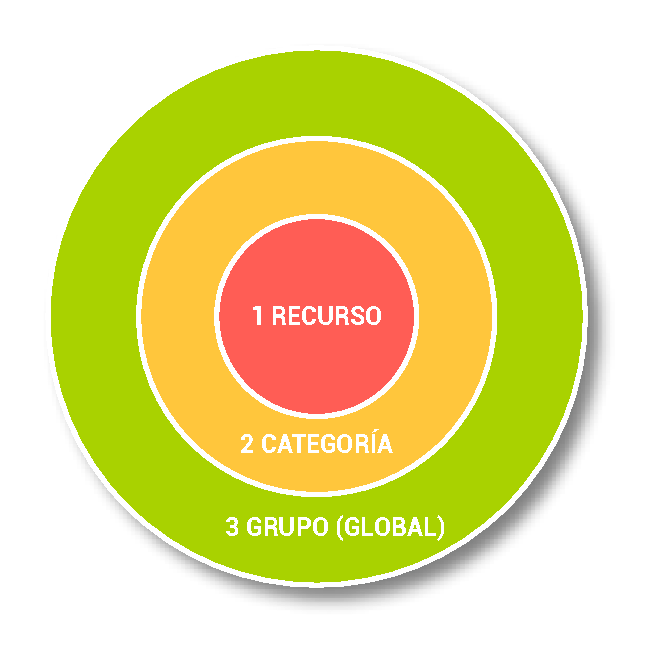
\includegraphics[width=.8\linewidth]{../graphics/fig_esquema_permisos_circular.eps}
\caption{Orden en el que se aplican los permisos en \tiki{}. Imagen inspirada en la documentación oficial \url{http://twbasics.keycontent.org/img/wiki_up/tiki_permissions.png}.}\label{fig:esquema_permisos_circular}
\end{figure}

\begin{itemize}
\item \textit{Recurso}: Los permisos de un recurso definen que acciones puede realizar un usuario para un recurso en concreto. Por ejemplo, podríamos tener una página \textit{wiki} que \textsc{no} permitiese subir ficheros, o que \textsc{no} permitiese la edición de su contenido, y dichos permisos serían los que imperasen, independientemente de que dicha \textit{wiki} estuviese categorizada en una categoría que permite editar contenidos \textit{wiki} o subir ficheros o de que el grupo, en general, pueda hacerlo.

 \item \textit{Categoría}: Los siguientes permisos en tenerse en cuenta son los relativos a que el recurso pertenezca a una categoría. Si, por ejemplo, en la categoría se describe que \textsc{no} se pueden subir imágenes a las páginas \textit{wikis} de esa categoría, y en cualquier página \textit{wiki} no existe un permiso que contradiga dicha regla, entonces se podrán subir imágenes. Recordamos que no puede existir un recurso que no esté asignado a ninguna categoría ya que, por defecto, pertenece a la categoría \texttt{Top} y dicha categoría también tiene unos permisos por omisión (que podemos modificar si así deseamos).

 \item \textit{Grupo (y los permisos globales)}: Los permisos de grupo son los últimos en aplicarse y son los que menos preferencia tienen en caso de que existan permisos contradictorios en los de categoría y los de recurso. Por otra parte, como cualquier usuario pertenece a un grupo, bien sea \texttt{Registered} o \texttt{Anonymous} sin contar con que esté en otros grupos se garantiza que, como mínimo, haya unos permisos globales básicos.  
\end{itemize}

A modo de resumen de lo expuesto anteriormente podemos decir que, si no hay una contradicción en los permisos, estos se heredan de arriba a abajo, es decir, Grupo \char"25B7~ Categoría \char"25B7~ Recurso. En cambio, si hay algún permiso que contradiga alguno de los anteriores, éstos sobreescriben de abajo a arriba, es decir, Grupo \char"25C1~ Categoría \char"25C1~ Recurso.

Si queremos obtener más información para administrar los permisos de las categorías, debemos acudir a la siguiente dirección: \url{http://localhost/tiki-admin_categories.php}.

\begin{figure}
\centering

\includegraphics[width=.8\linewidth]{../graphics/fig_asignacion_permisos_llave_verde.png}
\caption{Listado de todas las categorías disponibles. Para editar los permisos de una categoría hay que pinchar en el icono de la llave verde.}\label{fig:asignacion_permisos_llave_verde}
\end{figure}

\begin{figure}
\centering
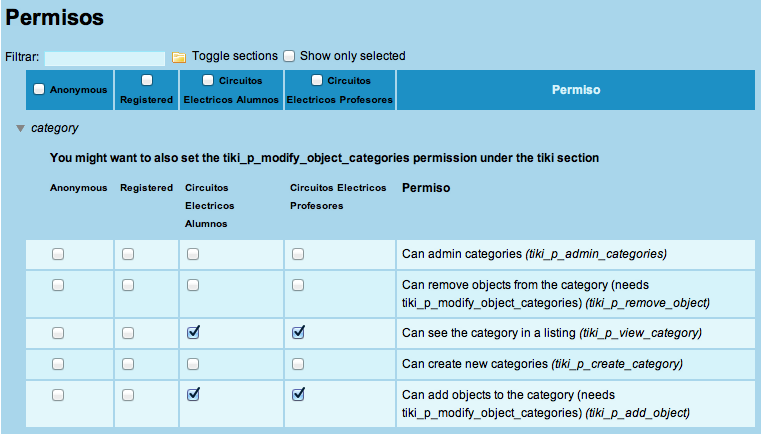
\includegraphics[width=\linewidth]{../graphics/fig_asignacion_permisos_categoria.png}
\caption{Listado de los posibles permisos que se pueden asignar a la categoría (en la imagen no se muestra toda la información). Como se puede apreciar, se pueden asignar permisos de manera independiente para cada grupo.}\label{fig:asignacion_permisos_categoria}
\end{figure}

\subsection{Concepto de preferencias}
\label{section:concepto-preferencias}

Como ya se ha comentado anteriormente, \tiki{} posee más de 1500 configuraciones y opciones posibles divididas en varios paneles de administración. Las \textit{preferencias} (como su propio nombre indica) nos permiten  configurar la plataforma a nuestro gusto. Será una tarea del administrador decidir qué \q{características} desee que estén activas, pasando por los recursos, como por la configuración de los envíos de correo a los usuarios, que apariencia externa tiene la plataforma, etcétera.

Uno de los problemas que plantea \tiki{} respecto a la administración es que tiene demasiadas posibilidades de configuración. Hay demasiados paneles, demasiadas casillas para activar y desactivar y múltiples opciones. Normalmente la tarea de configurar la plataforma se suele realizar la primera vez que se instala en el servidor. Este proceso puede incluso hasta llevar varias horas en completarse dependiendo, claro está, de las necesidades concretas de cada instalación y de la pericia que tenga manejando el \textit{software} el administrador.

Las principales desventajas que encontramos, aparte de la pérdida de tiempo que supone configurar, es que un usuario tiene que conocerse bien la plataforma (o al menos haber leído mucha información, o haber probado a base de ensayo y error). Además, las configuraciones no se pueden reutilizar, es decir, si disponemos de dos plataformas y queremos compartir la configuración que tenemos en una y llevarla a la otra de forma directa, no vamos a ser capaz de poder hacerlo.

Por fortuna los \profiles{} solventan de manera elegante todos estos inconvenientes y en el \chapterref{gestion-dinamica} veremos como se ha creado un \profile{} que configura \alma{} en muy poco tiempo. Pero para ello, antes debemos conocer un poco el funcionamiento básico de las preferencias en \tiki{}.

De forma interna las preferencias se guardan en tres tablas importantes de la base de datos que hay que conocer:

\begin{itemize}
 \item \texttt{tiki\_preferences}
 \item \texttt{tiki\_perspective\_preferences}
 \item \texttt{tiki\_user\_preferences}
\end{itemize}

\begin{figure}
\centering
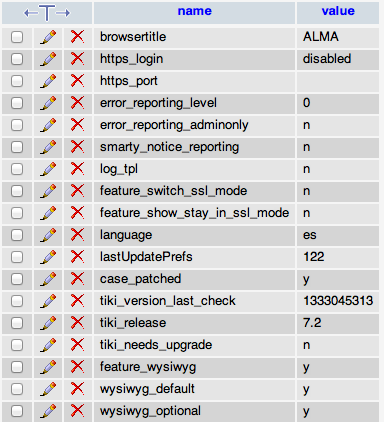
\includegraphics{../graphics/fig_valores_preferencias.png}
\caption{Algunos valores almacenados en la tabla \texttt{tiki\_preferences}.}\label{fig:valores_preferencias}
\end{figure}

La principal y la más importante es la tabla \texttt{tiki\_preferences}, ya que, es la encargada de almacenar los valores principales de todas las posibles configuraciones que pueden existir en \tiki{}. Dicha tabla almacena por ejemplo: el idioma que debe mostrar la aplicación, las \q{características} que hay habilitadas, la configuración para el envío de notificaciones de correo, el nombre de la plataforma\ldots{} Es decir, cualquier opción que modifiquemos en el panel de administración queda almacenado ahí.  
La estructura relacional de esta tabla es sencilla: almacena el nombre de la preferencia y su valor asociado.

\begin{figure}[h!]
\begin{pyglist}[language=sql]

  CREATE TABLE `tiki_preferences` (
    `name` varchar(40) NOT NULL default '',
    `value` text,
    PRIMARY KEY (`name`)
  ) ENGINE=MyISAM;
  
\end{pyglist}
\caption{Estructura de la tabla \texttt{tiki\_preferences}.}
\end{figure}
  
La librería de código que se encarga de almacenar y recoger los datos guardados en dicha tabla se llama \texttt{Prefslib.php} y dicho \textsc{php} se encuentra en la carpeta \texttt{lib/} al descargar el código fuente\footnote{Para más información sobre como está organizado el código fuente de \tiki{} recomendamos al lector la lectura del \appendixref{organizacion-codigo} al final del documento.}.

De forma genérica, y sin entrar en detalles muy concretos, cuando un usuario realiza una petición a \tiki{} esa librería extrae los datos de la tabla \texttt{tiki\_preferences} y los almacena en un \texttt{array asociativo} \cite{web:documentacion-php-arrays}. De esta manera podemos obtener los valores que deseemos utilizando una simple sentencia de programación de \php{}:

\begin{figure}[h!]
\begin{pyglist}[language=php]

  <?php
  print($prefs['tiki_release']); // Y obtendríamos el número de versión de TikiWiki.
      
\end{pyglist}
\caption{Un ejemplo de lo que contiene el array \code{\$prefs} (que son todos los datos de la tabla \texttt{tiki\_preferences}).}
\end{figure}

La tabla \texttt{tiki\_user\_preferences}, como su nombre indica, guarda, de manera análoga a como lo hace \texttt{tiki\_prerefences}, las preferencias que tienen los usuarios. Esto les permite configurar a cada uno que opciones desean de manera individual, es decir, cada usuario tiene sus propias preferencias. Por ejemplo: uno se podría llamar Pepito Pérez y su alias \texttt{pperez} y otro John Doe y su alias \texttt{jdoe} y esos datos se guardan en esa tabla.

La tabla \texttt{tiki\_perspective\_preferences} funciona de manera análoga a las anteriores, pero, su uso es diferente puesto que está ligado al concepto de las perspectivas. En la siguiente sección hablaremos más detalladamente de esta última tabla.

Tener un conocimiento de como se almacenan las preferencias y como se emplean nos ayuda posteriormente a poder desarrollar mejor los \profiles{} que configuren una instalación de \tiki{}.

Hay que decir que este tipo de información no se encuentra en ninguno de los canales oficiales presentados, por lo que recomendamos al lector interesado que explore de manera profunda lo que se ha presentado aquí si quiere obtener un conocimiento avanzado de como funciona internamente \tiki{}.

\subsection{Concepto de perspectivas}
\label{section:concepto_perspectivas}

\begin{figure}
\centering
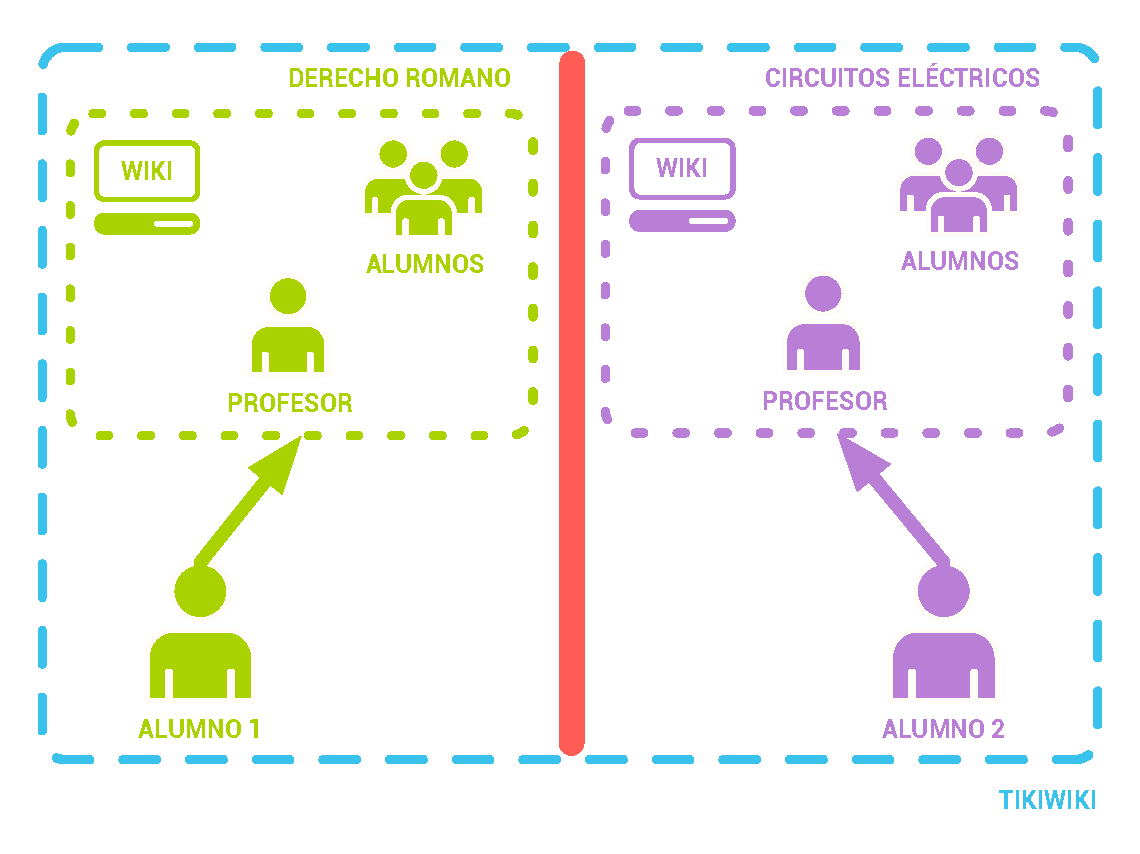
\includegraphics[width=.8\linewidth]{../graphics/fig_comunidad_de_practica_perspectivas.eps}
\caption{Ejemplo de dos posibles alumnos en el cual el Alumno 1 desconoce que existe la comunidad de práctica de Circuitos. Las perspectivas en \tiki{} nos permiten aislar de forma transparente comunidades de práctica dentro de una misma instalación.}\label{fig:comunidad_de_practica_perspectivas}
\end{figure}

Las \textit{perspectivas} son un concepto que apareció en las últimas versiones de \tiki{} (concretamente en la versión 4) y con las cuales somos capaces de implementar la separación entre diferentes comunidades de práctica utilizando la misma instalación de \textit{software}. Esto nos interesa mucho a la hora de implementar las comunidades de práctica, ya que, de esta manera podemos hacer que \tiki{} muestre solo cosas relevantes a un determinado grupo y no a otro (a un alumno concreto no le importa ver otras asignaturas que no sean a las que él está matriculado, \figureref{comunidad_de_practica_perspectivas}).

Además, aparte de separar diferentes comunidades de práctica, las perspectivas nos permiten personalizar \tiki{} y adaptarlo a las necesidades concretas de cada asignatura. Por ejemplo: en la vida real cuando un alumno entra en un aula puede encontrar un determinado color de pared, la distribución de las sillas tienen una forma determinada, la iluminación se manifiesta de una forma concreta\ldots{} y todas estas características son completamente diferentes en otro aula. Podemos replicar de manera \q{psicológica} este mismo comportamiento cambiando por ejemplo el logotipo principal de \tiki{} por el de la asignatura Circuitos cuando el alumno entra dentro de la comunidad de práctica, o cambiar el color del tema visual que se está utilizando por ejemplo de azul a verde. Lo positivo es que estos \q{efectos} duran mientras el usuario esté dentro de una comunidad de práctica, cuando la abandona, los cambios se revierten a los que había previamente (al igual que cuando un alumno abandona un aula el entorno previo permanece igual, \figureref{explicacion_perspectivas}).

\begin{figure}
\centering
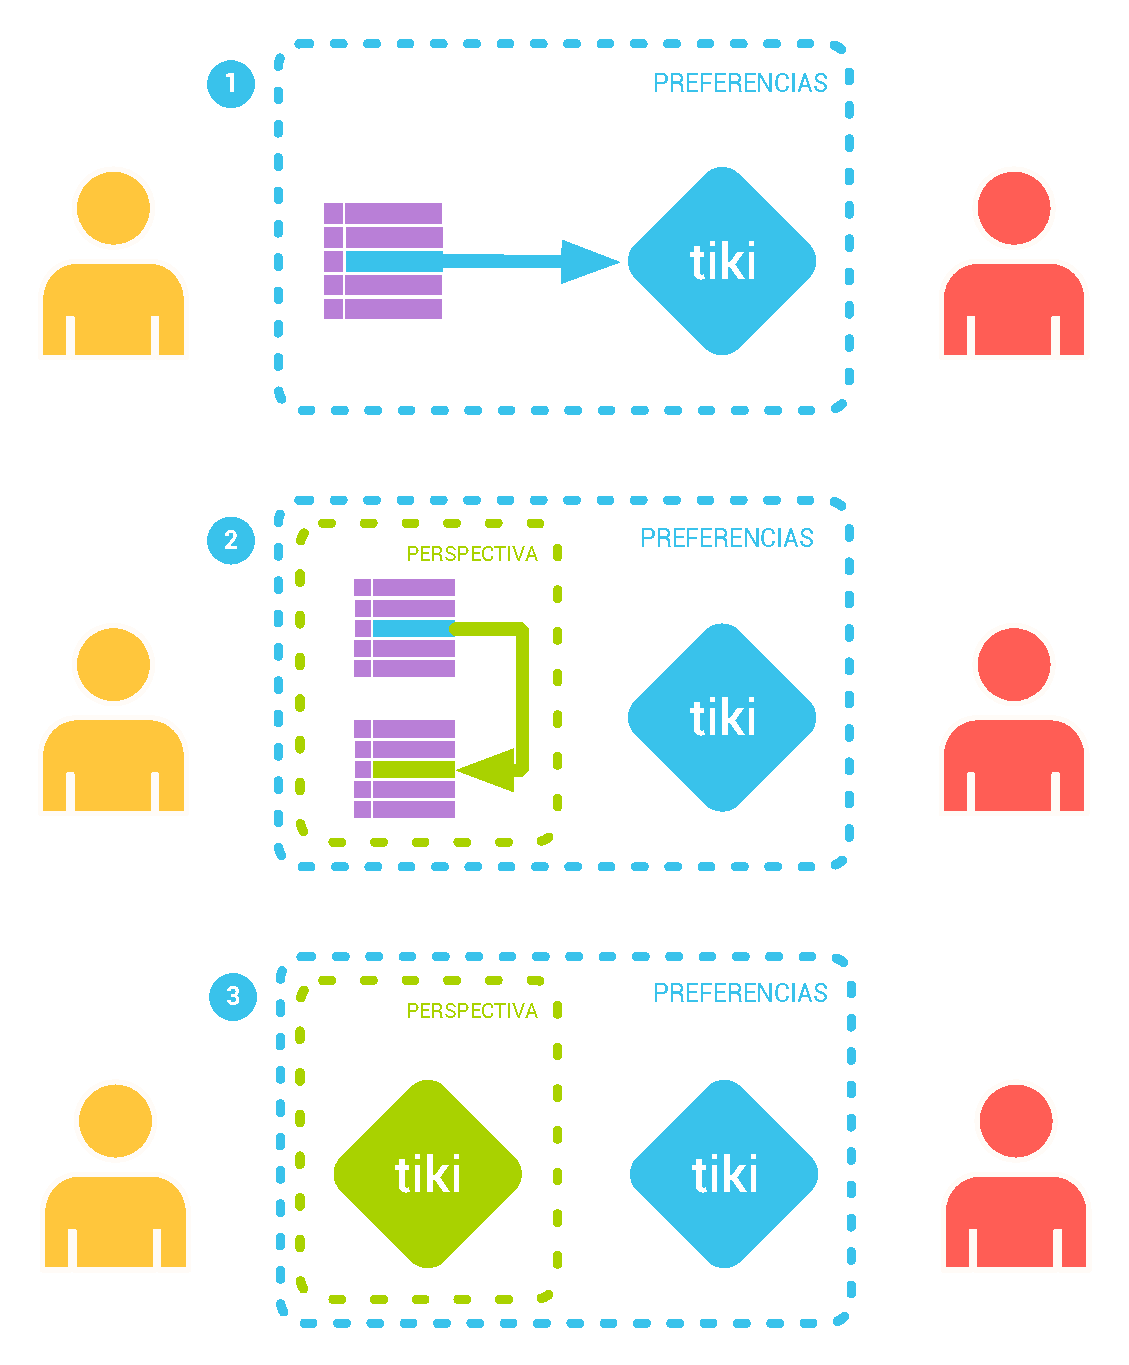
\includegraphics[width=.9\linewidth]{../graphics/fig_explicacion_perspectivas.eps}
\caption{Supongamos que existen dos usuarios y que pertenecen a dos comunidades de práctica diferentes. En el primer ejemplo (denotado en el gráfico con el número uno) los dos ven el color del logotipo de \tiki{} azul, ya que, así lo indica sus preferencias genéricas. En un instante de tiempo \texttt{t + 1} el usuario amarillo decide entrar en una comunidad de práctica. Dicha comunidad de práctica posee una perspectiva que cambia la preferencia de que el logotipo sea de color azul a que sea verde (se puede observar en el gráfico número dos como se ejecuta el cambio internamente). El usuario amarillo acaba entrando en la comunidad de práctica (gráfico número tres) y ya lo que él observa es que el logotipo ha cambiado de color, sin embargo, para el usuario de color rojo al no pertenecer a la misma comunidad de práctica (y, por consiguiente ,al no haber ejecutado la perspectiva asociada) observa que el color del logotipo sigue siendo azul. En el momento en el que el usuario amarillo abandone la comunidad de práctica, todos los cambios que ha efectuado la perspectiva se revierten y se volvería a estar en el gráfico número uno.}\label{fig:explicacion_perspectivas}
\end{figure}

El funcionamiento de las perspectivas es sencillo, simplemente sobreescriben temporalmente cualquiera de las 1500 preferencias que existen en \tiki{}. Recordamos al lector que las preferencias se guardaban en la tabla \texttt{tiki\_preferences}. Éstas en el momento en el que se activan, cargan y ejecutan las preferencias modificadas de la tabla \texttt{tiki\_perspective\_preferences}. Por lo tanto es importante saber que cualquier preferencia que exista en la tabla \texttt{tiki\_preferences} es susceptible de ser modificada por una perspectiva\footnote{Esto es importante saberlo ya que a la hora de implementar \profiles{} en la documentación oficial de \tiki{} no se listan todas las opciones posibles. La mejor solución es acudir a la tabla de las preferencias y ver que valores hay ahí.}. 

Las perspectivas pueden ser administradas desde la interfaz de \tiki{}, si el administrador visita el siguiente enlace: \url{http://localhost/tiki-edit_perspective.php} se encontrará con lo que muestra la \figureref{panel_administracion_perspectivas}; si decide editar las preferencias que modificará una perspectiva entonces verá lo que muestra la \figureref{detalle_modificacion_preferencias}.

\begin{figure}
\centering
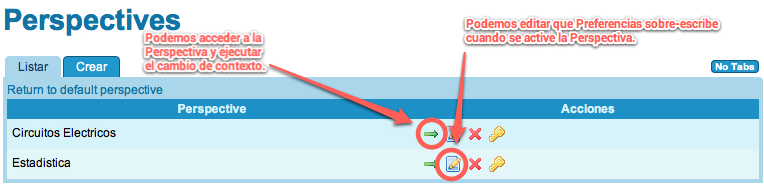
\includegraphics[width=\linewidth]{../graphics/fig_panel_administracion_perspectivas.png}
\caption{\tiki{} permite crear, editar y borrar perspectivas. Hay que reconocer que la interfaz web no es la forma más cómoda de administrar las perspectivas, aunque para ediciones sencillas sirve perfectamente.}\label{fig:panel_administracion_perspectivas}
\end{figure}

\begin{figure}
\centering
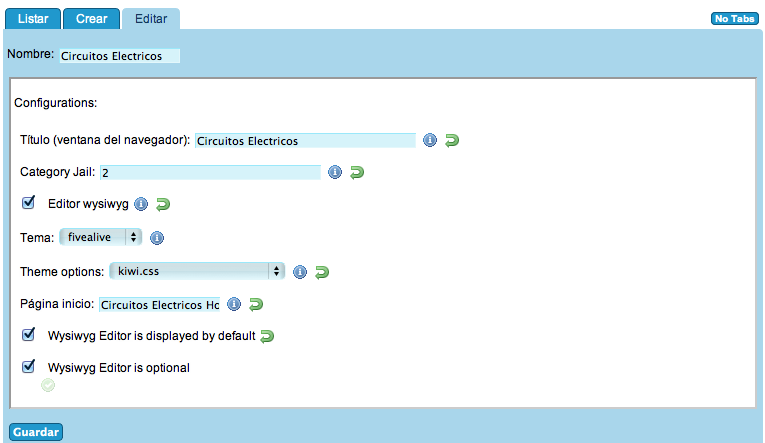
\includegraphics[width=\linewidth]{../graphics/fig_detalle_modificacion_preferencias.png}
\caption{Aquí se listan las preferencias que se activarán en la comunidad de práctica de la asignatura de Circuitos Eléctricos. Han sido generadas de forma automática con un \profile{} (añadir preferencias de forma manual es un proceso tedioso).}\label{fig:detalle_modificacion_preferencias}
\end{figure}

Para encontrar más información relativa a las perspectivas nada mejor que acudir a la documentación oficial \url{http://doc.tiki.org/Perspectives}.

\subsection{Concepto de menús}

\begin{figure}
\centering
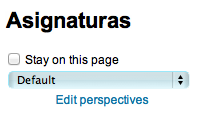
\includegraphics{../graphics/fig_menu_perspectivas.png}
\caption{Ejemplo de menú que se puede utilizar para cambiar las perspectivas y cambiar de comunidad de práctica de manera dinámica.}\label{fig:menu_perspectivas}
\end{figure}

\tiki{} tiene un gestor de creación de menús de manera que podemos generar menús que en nuestro caso nos permiten cambiar de manera dinámica las perspectivas y listar a las comunidades de práctica a las que pertenece el usuario. Esto nos permite que el usuario cambie de comunidad de práctica de manera rápida y sencilla, y al activarse la perspectiva asociada a dicha comunidad, cambiará la experiencia en \tiki{} de manera acorde. Es como si un alumno cambiase de aula (\figureref{menu_perspectivas}).

Por otra parte los menús tienen mucho más usos que para listar simplemente perspectivas. Si queremos administrar y crear menús, debemos ir a la siguiente dirección: \url{http://localhost/tiki-admin_menus.php} (\figureref{admin_menus}).

\begin{figure}
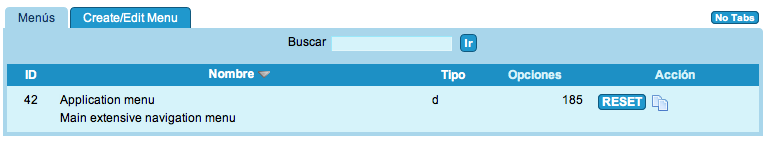
\includegraphics[width=\linewidth]{../graphics/fig_admin_menus.png}
\caption{Panel de administración de menús. Se pueden crear, editar y borrar. Hay una cantidad inmensa de opciones, más información en \url{http://doc.tiki.org/Menu+HOWTO}.}\label{fig:admin_menus}
\end{figure}

\section{¿Qué hemos aprendido de todo lo comentado en el capítulo?}

A lo largo de este capítulo hemos hecho un recorrido a las características más importantes que tiene \tiki{} que nos sirven para implementar una comunidad de práctica\footnote{De hecho en la documentación oficial de \tiki{} encontramos el concepto de \texttt{Workspaces} (\url{http://doc.tiki.org/Workspace}) que es básicamente lo que nosotros hemos denominado como comunidades de práctica. Y uno de los ejemplos es la creación manual de un \texttt{Workspace} similar a lo que hemos realizado aquí.}. Si bien, en cada sección no se ha profundizado con mucho detalle, en parte, porque si no se podrían rellenar muchas hojas presentando conceptos que el lector será capaz de descubrir fácilmente en el momento que decida utilizar la plataforma. Aún así, podemos extraer una idea importante: crear comunidades de práctica conlleva mucho tiempo y es una tarea en la que se pueden cometer errores fácilmente, puesto que, la complejidad crece de manera lineal conforme haya más comunidades de práctica a crear. Y eso, sin mencionar de tener que administrar dichas comunidades. Por lo tanto, los \profiles{} se postulan como una herramienta útil que nos ahorra tener que crear todas estas opciones de manera manual. En la siguiente parte descubriremos todo lo necesario para poder conseguir nuestro objetivo principal: liberar al administrador de las tareas repetitivas y aburridas.

      
    \part{Automatización de recursos con Profiles}
      \chapter{Profiles} 
\label{chapter:profiles}

\begin{center}

\includegraphics[scale=0.4]{../graphics/johnny_automatic_Jack_victorious.eps}
\end{center}

\lettrine{A}{lo largo de todo} este \pfc{} se han mencionado los \profiles{} en múltiples ocasiones y lo útiles que son o lo bien que encajan con el concepto de crear comunidades de práctica de una forma rápida y cómoda para un administrador o docente. Pero es aquí, en este capítulo, en el que se tratará de explicar de manera profunda qué son y cómo funcionan. Para lograrlo, se ha hecho una división del mismo en dos partes fundamentales: en la primera, veremos la teoría básica que sustenta los \profiles{}, primero a vista de pájaro, es decir, entenderemos el concepto y aprenderemos a manejar la herramienta en \tiki{} utilizando para ello un ejemplo real; en la segunda, se darán breves detalles técnicos de la implementación interna, es decir, del código fuente responsable del funcionamiento por si el lector desea modificar la herramienta a sus necesidades concretas. 

\section{¿Por qué surgen los Profiles?}

\tiki{}, al ser un \textit{software} muy completo, posee muchas características implementadas en su interior. Como usuarios de la plataforma podemos tomar ventaja de dicha arquitectura para construir casi cualquier cosa que deseemos. Pero, por norma general, resulta que muchas veces no queremos utilizar todas las herramientas que tenemos disponibles para implementar todos los posibles casos de uso que existen, si no que, dependiendo de nuestras necesidades específicas, modificamos la plataforma para realizar algo en concreto (utilizamos un subconjunto de ella). Por ejemplo: podríamos querer usar \tiki{} como un sistema para administrar nuestro \textit{blog}, o para hacer una \textit{wiki} corporativa para uso interno de la empresa en la que trabajamos, o para crear un foro de una comunidad de amantes del motor\ldots{} Como ya se ha comentado anteriormente, somos nosotros quienes ponemos límites a lo que queremos realizar.

Pero, uno de los problemas que ha arrastrado \tiki{} desde sus primeras versiones y hasta hace bien poco es que, con todas las características que posee la plataforma, ¿cuál es la mejor forma de estructurar los paneles de administración de una manera eficiente y que promueva la facilidad de uso entre sus usuarios? La respuesta a esta pregunta es que los desarrolladores de \tiki{} todavía no lo han conseguido (si, incluso hasta en las versiones más modernas siguen adoleciendo de este problema). A lo largo de la vida del proyecto han modificado, en varias ocasiones, los paneles de administración para hacerlos más intuitivos, pero, 1500 opciones de configuración posibles son demasiadas opciones a tener en cuenta. Esto hace que cualquier usuario que quiera manejar la plataforma tenga que dedicar una considerable cantidad de tiempo en aprender las entrañas del programa. Además otro problema, análogo al anterior, es que no sólo existen los paneles de administración principales (como los que vimos en el \chapterref{conceptos-fundamentales-tiki}), si no que también hay otros paneles secundarios (también dedicados para propósitos administrativos) que están distribuidos por diferentes partes de la plataforma.

Debido a los inconvenientes expuestos, a partir de la versión 4 de \tiki{}, se decidió hacer una reescritura masiva de todas las librerías principales y se comenzó a trabajar con el proyecto de los \profiles{}. A día de hoy, y en la versión 8, todavía continúan integrando y mejorando esta herramienta. Lo que está claro es que es una parte importante de la plataforma y así lo seguirá siendo en los próximos años, ya que, los \profiles{} solucionan el problema conocido como: \textit{la paradoja de la elección}\footnote{Esta teoría fue propuesta por Barry Schwartz en su libro \work{The Paradox of Choice: Why More Is Less} donde plantea que el exceso de opciones nos lleva a la parálisis y a la inacción. Y el problema posterior que surge: ansiedad, cuando hemos elegido \cite{libro:la-paradoja-de-la-elección}.}.

\section{¿Qué son los Profiles?}

Un \textit{Profile} no es más que un archivo de texto (que se encuentra almacenado en una página \textit{wiki} normal y corriente) con una serie de instrucciones que explican, paso a paso, que deseamos modificar de cualquiera de las 1500 preferencias de \tiki{}, permitiéndonos también, el poder crear, cambiar y borrar cualquier recurso que queramos. Para ello, hay una herramienta dentro de la librería de los \profiles{} encargada de traducir el texto contenido en una página \textit{wiki} en acciones concretas de la plataforma (\figureref{flujo_accion_profile}).

\begin{figure}[h!]
\centering
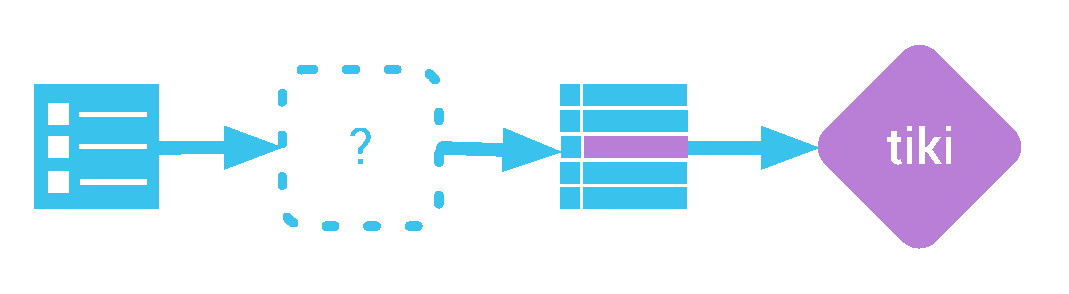
\includegraphics[width=\linewidth]{../graphics/fig_flujo_accion_profile.eps}
\caption{Un \profile{} \textit{modifica} las preferencias de \tiki{} de la manera en la que esté especificado. El rectángulo con el interrogante es el traductor que se encarga de \q{entender} lo que el \profile{} desea alterar (veremos más detalles internos en la \sectionref{componentes-profiles}).}\label{fig:flujo_accion_profile}
\end{figure}

Si recordamos nuestro periplo por el \chapterref{conceptos-fundamentales-tiki}, buena parte de éste se dedicó a explicar muchos conceptos \textit{críticos} de \tiki{} a la vez que se demostraban cuales eran los pasos que tenía que seguir un administrador para poder crear \textit{una} comunidad de práctica.
En lugar de tener que lidiar con los paneles de administración, una opción es que podemos concebir un \profile{} que explique, como si de una receta de cocina se tratase, como se debe crear una comunidad de práctica (\figureref{etapas_profile}). (Y De esta manera podemos automatizar un proceso que es de índole repetitiva.)

\begin{figure}[h!]
\centering
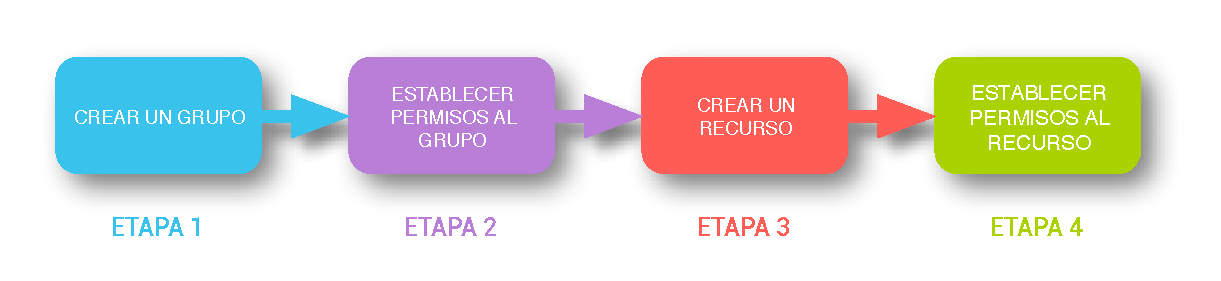
\includegraphics[width=\linewidth]{../graphics/fig_etapas_profile.eps}
\caption{Para cada \profile{} hay que definir exactamente que deseamos ejecutar. Una forma de crear un \profile{} con éxito es dividir lo que queremos crear en etapas.}\label{fig:etapas_profile}
\end{figure}

La parte buena del asunto es que, con los \profiles{}, al ser realmente páginas \textit{wiki} podemos hacer que la comunidad (o cualquier persona) participe en compartirlos o en mejorar los ya existentes (y ya no sólo son útiles para crear comunidades de práctica si no para cualquier otra tarea). De esta forma se aumenta el número de casos de uso a los que podemos configurar \tiki{} y se facilita la reutilización de código ya que algo que deseemos realizar, con toda certeza, habrá sido pensado por alguien antes que nosotros.

\subsection{Beneficios que aportan los Profiles a TikiWiki}

En la documentación oficial de los \profiles{} se listan algunas de las características y ventajas que llevan consigo la utilización de dicha herramienta en \tiki{} (se han adaptado y expandido ciertas ideas, la mayoría se han expuesto anteriormente) \cite{web:explicacion-profiles}:

\begin{itemize}
\item Son sencillos de almacenar. Un \profile{} es un archivo de texto plano que puede ser almacenado en las propias páginas \textit{wiki}.

\item Facilitan la colaboración, ya que, al ser guardados en forma de páginas \textit{wiki} podemos utilizar todas las ventajas que nos proporcionan estas herramientas, como por ejemplo: múltiples versiones de un \profile{} gracias al historial de ediciones que incorpora la \textit{wiki}.

\item Pueden modificar cualquier preferencia que exista en \tiki{} como todas las que se almacenan en la tabla \texttt{tiki\_preferences} (\sectionref{concepto-preferencias} en el \chapterref{conceptos-fundamentales-tiki}); también pueden crear nuevos recursos (\sectionref{concepto-recursos} del mismo capítulo) y asignar o modificar cualquier tipo de permiso de los existentes en \tiki{} en cualquier ámbito (ya sea de recurso, de categoría o de grupo).

\item Permiten la ejecución simultánea de varios \profiles{} y se pueden ejecutar en cualquier momento que deseemos. Si alguno de los \profiles{} que ejecutemos en paralelo genera conflictos con otro, la configuración del último ejecutado es prioritaria, es decir, evitan dejar a \tiki{} mal configurado.

\item Composición. Los \profiles{} admiten adjuntar otros \profiles{} dentro de un \profile{}, es decir, se puede construir uno gigante con la unión de varios pequeños. También un mismo \profile{} puede ser dividido en múltiples fragmentos y entre ellos insertar sintaxis \textit{wiki}.
\end{itemize}

\subsection{Beneficios que aportan los Profiles a \textsc{alma}}

Nosotros hemos decidido utilizar los \profiles{} por dos motivos principalmente:

\begin{enumerate}
\item Crear comunidades de práctica. Dado que este es el interés principal de este \pfc{}, los \profiles{} encajan muy bien con lo que queremos hacer, puesto que, permiten, en un sólo segundo, tener preparado una comunidad de práctica para cualquier asignatura.

\item Configurar la plataforma de \alma{}. Dado que el proyecto tiene unas necesidades muy concretas, la propia configuración de éste es una tarea que se realiza muy bien con un \profile{}. De esta forma podemos replicar múltiples \q{\textsc{almas}} en poco tiempo.
\end{enumerate}

\section{Flujo de trabajo con los Profiles}
\label{section:componentes-profiles}

El flujo de trabajo con \profiles{} es bastante intuitivo una vez que se tienen claro algunos conceptos importantes. Para ello, vamos a ampliar el contenido mostrado en la \figureref{flujo_accion_profile} y también a dividirlo en pequeñas etapas que expliquen cada apartado de manera clara y concisa. Recomendamos al lector observar detenidamente la \figureref{flujo_trabajo_profiles}, pues, contiene una visión general de cada etapa:

\begin{figure}[h!]
\centering
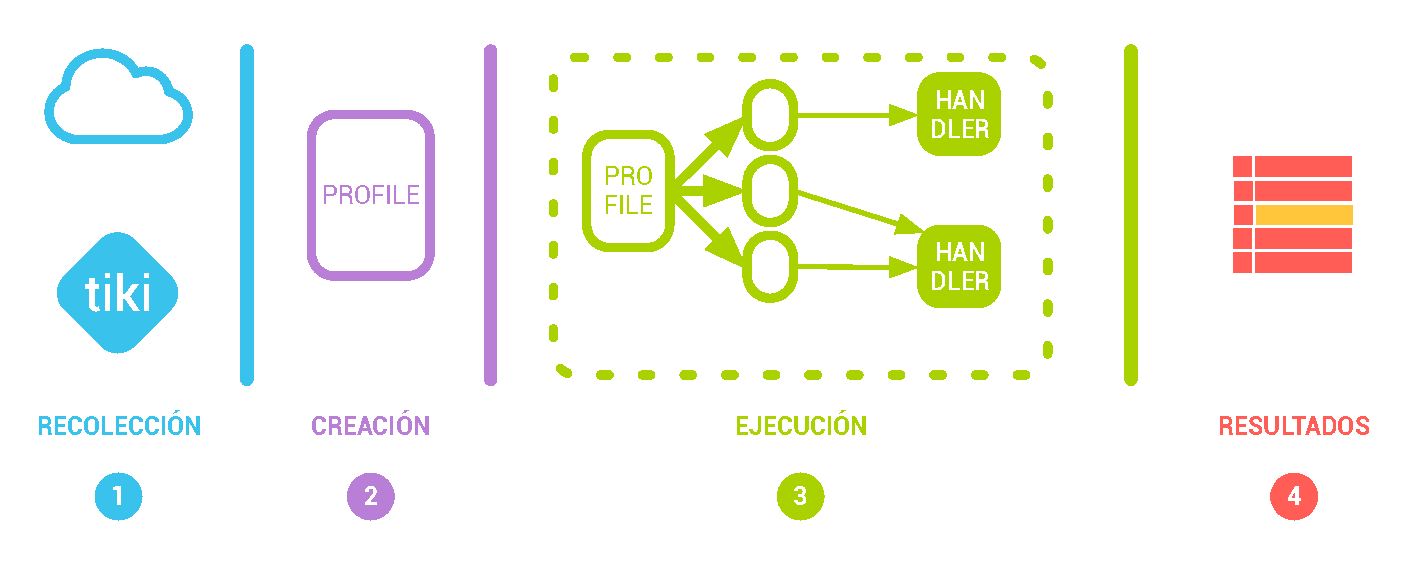
\includegraphics[width=\linewidth]{../graphics/fig_flujo_trabajo_profiles.eps}
\caption{}\label{fig:flujo_trabajo_profiles}
\end{figure}

\subsection{Recolección}

Una vez que hemos decidido trabajar con los \profiles{}, y sobre todo para esta primera estapa, debemos efectuarnos la siguiente pregunta: \q{¿Obtenemos un \profile{} que ya esté hecho o lo creamos desde cero?} 
Dependiendo de la respuesta, el flujo de trabajo puede variar ligeramente: si descargamos un \profile{} prefabricado hay que conseguirlo de algún lado mientras que, si lo creamos desde cero, no habría que hacer nada más (nos tendríamos que poner a escribir lo que deseamos crear, pero, sin depender de nada ni de nadie).

Para obtener un \profile{} que ya está diseñado de antemano, \tiki{} utiliza el concepto de \textit{repositorios}\footnote{El concepto de repositorio en \tiki{} se asemeja bastante, en idea, a los gestores de paquetes que se utilizan en varias distribuciones de Linux como: \texttt{apt} \cite{web:apt-debian}, \texttt{pacman} \cite{web:pacman-arch} o \texttt{yum} \cite{web:yum-fedora}.}. ¿Y qué son? Entendemos por repositorio aquel sitio centralizado donde se almacena y se mantiene un conjunto de \profiles{}. Se pueden clasificar en dos tipos:

\begin{itemize}
    \item \textbf{Externos}: Son en los que en nuestra instalación de \tiki{}, ésta necesita conectarse a un servidor externo para obtener un listado de todos los \profiles{} existentes. Por defecto, cuando instalamos \tiki{} por primera vez, nos añade el repositorio principal de \profiles{}: \url{http://profiles.tiki.org}. En dicho repositorio podemos encontrar todo tipo de \profiles{}, y éstos se pueden encontrar clasificados por funcionalidad, por número de versión, por la cantidad de votos que han recibido de otros usuarios que los han usado\ldots{} Pero también podemos optar por crear nuestro propio repositorio de \profiles{}, ya que, en el fondo son simplemente páginas \textit{wikis}.

    \item \textbf{Locales}: Son aquellos que se encuentran de manera local en nuestra plataforma y, por lo tanto, nuestra instalación de \tiki{} no necesita realizar ninguna petición a Internet. A su vez, se clasifican en dos formas: los que almacenan los \profiles{} en la misma instalación de \tiki{}, por ejemplo: \alma{} utiliza esta configuración\footnote{En la \sectionref{profile-creado-desde-cero} veremos que la ejecución de los \profiles{} de esta manera requieren un tratamiento especial, utilizan un componente añadido llamado \textit{Data Channel}.}; o replicar a su vez, una instalación de \tiki{} dedicada a \profiles{} (similar al repositorio oficial) pero en el que no hay un acceso a Internet. Por ejemplo: podría usarlo una empresa en una \textit{intranet} y separar así la instalación de trabajo de la del repositorio.
\end{itemize}

\subsection{Creación}

En esta segunda etapa, según la elección que hayamos tomado en la anterior, puede variar en la forma de llevarla a cabo: si decidimos obtener un \profile{} de algún repositorio es bastante probable que queramos ejecutarlo sin modificar nada de éste (aunque tenemos la opción de poder hacerlo); en cambio, si, por el contrario, hemos decidido crear un \profile{} desde el principio es, en esta etapa, en la que tenemos que pensar de manera creativa que queremos realizar con el mismo.

Cuando hablamos de un \profile{}, en concreto, nos estamos refiriendo al texto que encontramos dentro de una página \textit{wiki} y que es el que posee la información para que pueda ser evaluado por el intérprete de \profiles{} y que ejecute una acción (o varias) dentro de \tiki{}. Para poder crear uno hay que seguir unas reglas definidas: 

\begin{itemize}
    \item Utilizan un formato de marcado ligero llamado \yaml{}\footnote{Instamos al lector que si desconoce que es \yaml{} visite el \appendixref{yaml} para obtener unas nociones básicas, puesto que, los \profiles{} se basan en dicho formato y es necesario conocerlo para poder trabajar con ellos.} y, por lo tanto, el documento debe de estar conforme a esa especificación. Si no es así, el intérprete de \profiles{} lanzará un error informando al usuario de que no se ha podido leer correctamente el contenido del documento.

    \item Además, también tienen que ser escritos conforme a las reglas que dictaminen los \textit{Handlers} (los encargados de traducir la sintaxis \yaml{} en acciones concretas de \tiki{}, veremos más información en la \sectionref{ejecucion-profiles}).

\item Ya que los \profiles{} se almacenan en páginas \textit{wikis}, éstos pueden utilizar la potencia de la sintaxis \textit{wiki} y, por ejemplo: se puede dividir un \profile{} en múltiples partes y en cada una de ellas ir explicando su funcionamiento. O también, cada división puede ser un \profile{} que realice una tarea determinada. Lo importante es que cada bloque que pertenezca a un \profile{} debe de comenzar con \texttt{\{CODE(caption=>YAML)\}} y finalizar con \texttt{\{CODE\}}. A continuación, un ejemplo real que ilustra mejor los conceptos explicados:
\end{itemize}

\begin{figure}
\begin{pyglist}[language=text]
  Esto es un documento Wiki en el que ahora mismo utilizamos 
  la sintaxis wiki. A continuación en la siguiente linea 
  tenemos un bloque que marca el comienzo de un Profile.

  {CODE(caption=>YAML)}
  preferences: 
    feature_articles: y
  objects:
   -
    type: article_type
    ref: type
    data:
      name: New Type
      allow: [ ratings, comments ]
      show: [ author, reads, language ]
   -
    type: topic
    ref: topic
    data:
      name: New Topic
  {CODE}

  Podemos continuar editando nuestro documento con formato wiki 
  y cuando queramos, volvemos con un Profile que haga otra cosa
  (o que continúe con el anterior Profile).

  {CODE(caption=>YAML)}
  preferences: 
   feature_galleries: y
   feature_wiki: y
  {CODE}
\end{pyglist}
\caption{Ejemplo de una posible página \textit{wiki} con dos bloques de \profiles{}. Cada bloque puede realizar una tarea distinta o bien ser la misma tarea dividida en secciones y explicada por partes. Ejemplo extraído de: \url{http://profiles.tiki.org/Article+Handler}.}
\end{figure}

\subsection{Ejecución}
\label{section:ejecucion-profiles}

En las anteriores etapas se requería tomar ciertas decisiones que condicionaban, un poco, la manera de hacer las cosas frente a la creación de un \profile{}. En esta etapa, en cambio, no requiere ninguna interacción por parte del usuario ya que se realiza de forma automática cuando se ejecuta un \profile{}. Más bien nos sirve como excusa para presentar un concepto muy importante denominado: \textit{Handler}.

Un \textit{Handler} es un componente programado en la librería de \profiles{} que se encarga de leer y traducir a acciones reales (por ejemplo: crear una categoría, activar un recurso, asignar permisos\ldots{}) los bloques de texto que contengan sentencias de \profiles{} en una página \textit{wiki}. Actualmente hay dieciocho \textit{Handlers} cada uno encargado de realizar una tarea determinada, a saber:

\begin{itemize}
\item \textit{Article Handler}

\item \textit{Blog Handler}

\item \textit{Category Handler}

\item \textit{External Wiki Handler}

\item \textit{File Gallery Handler}

\item \textit{Forum Handler}

\item \textit{Menu Handler}

\item \textit{Module Handler}

\item \textit{Perspective Handler}

\item \textit{Plugin Alias Handler}

\item \textit{RSS Handler}

\item \textit{Template Handler}

\item \textit{Tracker Handler}

\item \textit{Transition Handler}

\item \textit{Webmail Handler}

\item \textit{Webservice Handler}

\item \textit{Wiki Handler}

\item \textit{Users Handler}
\end{itemize}

Cada uno tiene su propia sintaxis que se debemos respetar para que el intérprete de \profiles{} sea capaz de dar por bueno un \profile{} que hayamos escrito. Podemos encontrar toda la documentación referente a todas las posibles opciones que podemos poner visitando la documentación oficial \cite{web:handlers}. En la \figureref{ejemplo_opciones_handler_usuario}, se muestra las opciones que posee el \textit{Handler} de Usuarios (\textit{Users Handler}) y que podríamos utilizar para crear un \profile{} que implique la creación, de manera automatizada, de usuarios. Cabe añadir que la sintáxis no hace falta aprenderla de memoria, cuando tengamos alguna necesidad, simplemente hay que visitar la web y consultar lo que deseemos.

\begin{figure}
\centering
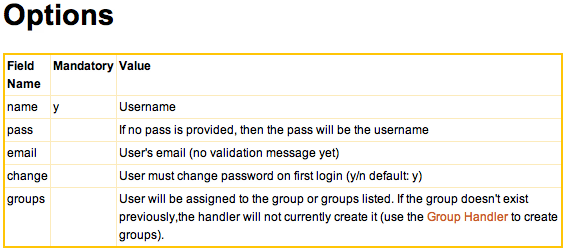
\includegraphics[width=\linewidth]{../graphics/fig_ejemplo_opciones_handler_usuario.png}
\caption{Estas son las opciones que se pueden poner en un \profile{} si queremos crear un usuario.}\label{fig:ejemplo_opciones_handler_usuario}
\end{figure}

\subsection{Resultados}

En esta etapa, la última, lo que obtenemos son los resultados de manera visible de lo que hayamos realizado con nuestro \profile{}. Ya sean cambios muy drásticos o, por contra, muy leves. A partir de aquí podemos repetir el flujo de trabajo con los \profiles{} desde el principio y tantas veces como deseemos, solo que en las siguientes veces, ya no tendremos que diseñarlo, pues, éste fue creado anteriormente.

\section{Explicación de la interfaz de los Profiles}

La administración de los \profiles{} por parte de un administrador es bastante simple y, prácticamente, no requiere de aprendizaje alguno. Si un usuario visita la siguiente dirección: \url{http://localhost/tiki-admin.php?page=profiles} lo que se encontrará es lo que se muestra en la \figureref{admin_profiles_pestaña_1} (un panel principal dividido en tres pestañas):

\begin{itemize}
    \item \textit{Ejecutar \profiles{} (Apply \profiles{})}: Mostrada en la figura anterior, esa pestaña es la encargada de listar todos los \profiles{} que ha encontrado \tiki{} en un determinado repositorio (sea el oficial o cualquier otro). Desde aquí el usuario puede elegir y filtrar, según preferencias, que tipos de \profiles{} desea ver. Tiene la opción de obtener más información acerca de lo que hace un \profile{} en concreto (que cosas crea y que cambia) y, por supuesto, de ejecutarlo en su instalción de \tiki{} (\figureref{ejecucion_profile}).

\item \textit{Exportar}: Esta pestaña permite al administrador volcar todos los datos de configuración que haya realizado sobre \tiki{}. Pero, ojo, ¡sólo las preferencias! Si se ha ejecutado anteriormente un \profile{} que genera grupos, por poner un ejemplo, no se guarda ni los grupos creados ni la información que contengan éstos (\figureref{exportar_configuracion_pestaña_2}).

\item \textit{Avanzado}: Aquí se pueden añadir nuevos repositorios, crear múltiples \textit{Data Channels} (como se dijo antes, entenderemos el concepto con un ejemplo práctico en la siguiente sección) y, en última instancia, existe un apartado para ejecutar los \profiles{} directamente. Esto nos sirve para probar configuraciones útiles o para realizar ejecuciones de prueba. Hay que tener especial cuidado porque como se indica en la imagen, se pueden hacer cambios irreversibles en la configuración de la base de datos (\figureref{pestaña_avanzado_3}).
\end{itemize}

\begin{figure}
\centering
\includegraphics[width=\linewidth]{../graphics/fig_admin_profiles_pestaña_1.png}
\caption{Panel principal de administración de los \profiles{}.}
\label{fig:admin_profiles_pestaña_1}
\end{figure}

\begin{figure}
\centering
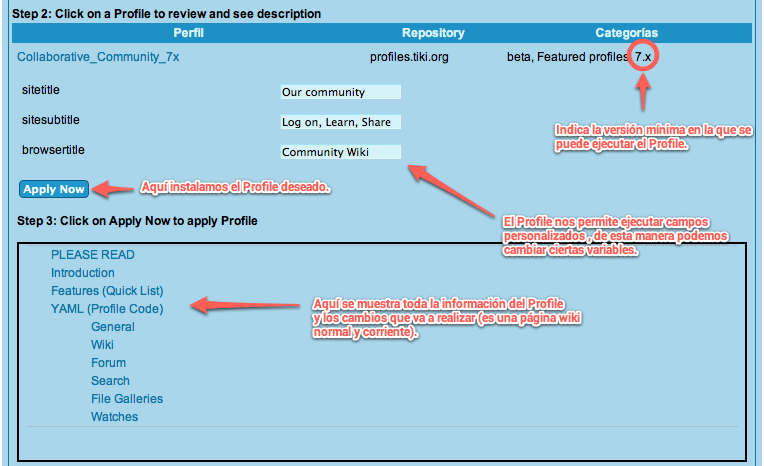
\includegraphics[width=\linewidth]{../graphics/fig_ejecucion_profile.png}
\caption{Panel donde podemos listar los \profiles{} que tiene un repositorio y ejecutarlos.}\label{fig:ejecucion_profile}
\end{figure}

\begin{figure}
\centering
\includegraphics[width=\linewidth]{../graphics/fig_exportar_configuracion_pestaña_2.png}
\caption{Panel donde podemos exportar las preferencias que hayamos modificado de \tiki{}. Se puede utilizar como método de copia de seguridad para restaurar posteriormente la misma configuración.}\label{fig:exportar_configuracion_pestaña_2}
\end{figure}

\begin{figure}[H]
\centering
\includegraphics[width=\linewidth]{../graphics/fig_pestaña_avanzado_3.png}
\caption{Panel que nos permite añadir nuevos repositorios, agregar nuevos \textit{Data Channels} y ejecutar \profiles{} de prueba.}\label{fig:pestaña_avanzado_3}
\end{figure}

\section{Un ejemplo con Profiles}

Vamos a mostrar dos ejemplos: uno sencillo y otro más complejo para entender mejor todos los conceptos que han sido presentados hasta ahora. En ambos casos, se pretende explicar al lector los pasos necesarios que tiene que seguir un hipotético administrador que desea crear, todo de manera automatizada, una página \textit{wiki} denominada \q{Prueba}, una categoría (también con el mismo nombre) en cuyo interior se encuentra la página anterior y, por último, cambiar el tema visual que utiliza \tiki{} (por defecto en azul) por otro en amarillo. La diferencia principal de los dos ejemplos estriba en la forma de llevarlo a cabo, en el primero, se asume que hay un \profile{} en el repositorio oficial. En el segundo, en cambio, se crea el \profile{} desde cero y se ejecuta en la instalación local utilizando para ello los \textit{Data Channels}.

\subsection{Profile ejecutado desde un repositorio}

Este es el caso más sencillo, los pasos son los siguientes:

\begin{enumerate}
\item Como administradores nos dirigimos a la página de administración de \profiles{} (recordemos: \url{http://localhost/tiki-admin.php?page=profiles}).

\item Listamos los \profiles{} existentes en el repositorio oficial y buscamos uno que se llama \texttt{Test\_Wiki\_Group} (podemos basarnos en las imágenes de la anterior sección puesto que este paso no cambia prácticamente nada, sólo el nombre del \profile{} a listar, \figureref{ejecucion_profile}).

\item Rellenamos las casillas con los nombres apropiados, el nombre de la página \textit{wiki}, el de la categoría y el del grupo y pulsamos ejecutar.

\item \textit{¡Et voilá!} Acción ejecutada, podemos comprobar en la \figureref{profile_ejemplo} que se cumple lo que el \profile{} prometía.

\end{enumerate}

\begin{figure}
\centering

\includegraphics{../graphics/fig_profile_ejemplo.png}
\caption{Categoría creada con una página wiki tal y como el Profile había especificado.}\label{fig:profile_ejemplo}
\end{figure}

\subsection{Profile ejecutado desde una instalación local}
\label{section:profile-creado-desde-cero}

En este caso, un poco más complejo, el \profile{} se ejecuta en una instalación local por lo que los pasos varían en varios puntos respecto al anterior ejemplo:

\begin{enumerate}

    \item Dado que en esta situación tenemos que crear el \profile{} desde cero, conviene pensar (como ya hicimos anteriormente) en términos absolutos: ¿qué queremos conseguir? y ¿cómo lo vamos a realizar? La respuesta a la primera pregunta está clara, lo definimos anteriormente: crear una página \textit{wiki} con un nombre determinado, una categoría de idéntico nombre que agrupe al anterior recurso y cambiar el color del tema visual. La respuesta para la segunda pregunta nos obliga a pensar en términos de \textit{Handlers}, en este caso, ¿qué \textit{Handlers} intervienen? Para crear la página \textit{wiki} es casi seguro que necesitaremos el \textit{Wiki Handler}, para la categoría utilizaremos el \textit{Category Handler} y para cambiar el color al ser una preferencia se puede poner directamente en el \profile{} (en la \figureref{listado_profile_ejemplo} tenemos de manera completa el \profile{} que utilizaremos, dejamos al lector la tarea de investigar y comprender las opciones que se listan utilizando para ello la bibliografía existente).

\item Una vez que tenemos claro como va a ser el \profile{}, hay que crear una página \textit{wiki} para almacenarlo, denominaremos a la página \textit{wiki} \texttt{primer\_profile} (no hay que olvidar este nombre ya que lo utilizaremos después y lo debemos respetar tal y como está escrito), copiamos el \profile{} (\figureref{listado_profile_ejemplo}), añadimos los fragmentos al principio (\texttt{\{CODE(caption=>YAML)\}}) y al final (\texttt{\{CODE\}}) del \profile{} y guardamos la página (\figureref{editar_primer_profile}).

\item Ya hemos creado la página \textit{wiki} con nombre \texttt{primer\_profile} y el \profile{} dentro. A partir de ahora podemos modificar la página tantas veces como queramos y recuperar su contenido con el historial de versiones.

\item Debido a que el \profile{} se va a ejecutar de manera local tenemos que utilizar los \textit{Data Channels} que es el encargado de avisar a \tiki{} para que no busque en otro repositorio externo, sino dentro de si mismo\footnote{Aunque los \textit{Data Channels} tienen más usos que el que se lista en este ejemplo. Si queremos ver todos y aprender más sobre ellos conviene visitar su página \textit{wiki} \cite{web:data-channels}.}. Para ello vamos a la pestaña de Avanzado en el panel de administración de \profiles{} (\figureref{pestaña_avanzado_3}) y tenemos que introducir lo siguiente en la casilla de \textit{Data Channels}:

\begin{pyglist}[language=text]
  mi_prueba, tiki://local, primer_profile, Admins
\end{pyglist}
 
La documentación de los \textit{Data Channels} explican el significado de cada elemento, un resumen:
\begin{itemize}
\item \textit{mi\_prueba}: Tenemos que denominar al \textit{Data Channel} con un identificador único, puede ser cualquier nombre que sea un carácter alfanumérico incluyendo también al símbolo \_.

\item \textit{tiki://local}: Indica a \tiki{} que utilice la página \textit{wiki} como \profile{} ya que está en su propia base de datos y no en un repositorio externo.

\item \textit{primer\_profile}: Indicamos a \tiki{} cual es la página en concreto que se usará como \profile{}. Se corresponde con el nombre que dimos a la página \textit{wiki} anteriormente.

\item \textit{Admins}: Especificamos que grupo tiene derecho a ejecutar el \profile{}. Se recomienda poner grupos que sean de confianza (es una imprudencia asignar el \profile{} a un grupo como \texttt{Anonymous} donde cualquiera puede ejecutarlo). Si queremos poner más grupos, se pueden poner separados por coma, por ejemplo: \texttt{Admins, Grupo1, Grupo2}.
\end{itemize}

\item Guardamos la información que hemos escrito en el \textit{Data Channel}. ¡La parte más difícil ya está superada! Ahora tenemos que buscar la manera de poder ejecutar el \profile{}, y para ello vamos a crear una interfaz gráfica con un botón al que siempre podamos acudir cuando queramos utilizar el \profile{} (en la \figureref{interfaz_plugin_data_channel} vemos un ejemplo de como quedaría al final del proceso). Para ello vamos a generar una nueva página \textit{wiki} denominada \texttt{mi\_profile\_interfaz} y copiaremos el contenido de la \figureref{datachannel} (en la descripción del mismo se explica el significado de todo el código).

\item ¡Y ya está! Cada vez que queramos utilizar dicho \profile{} acudimos a la página \texttt{mi\_profile\_interfaz} pulsamos el botón y este ejecuta el \profile{} guardado en \texttt{primer\_profile}. Hay que avisar que si un usuario que no pertenezca al grupo \texttt{Admins} (que así fue como lo especificamos en la linea de los \textit{Data Channel} en el paso 4) intenta ejecutar el \profile{}, éste no hará nada. No obstante un usuario que no esté autorizado a ejecutar \profiles{} no debería ver tampoco esta página así como donde está el \profile{} en sí (nos evitaremos muchos problemas a la larga).
\end{enumerate}

\begin{figure}
\begin{pyglist}[language=text]
  {CODE(caption=>YAML)}
  preferences: 
   style_option: kiwi.css
   enable: [ feature_wiki ]
  objects:
   -
    type: wiki_page
    data:
      name: Prueba
      content: Creando una wiki con profiles
      ref: pagina_prueba
   -
   type: category
    data:
     name: Prueba
     items:
      - [ wiki_page, pagina_prueba ]
  {CODE}
\end{pyglist}
\caption{En la sección de \code{preferences} se pueden poner las preferencias directamente que encontramos en la tabla \texttt{tiki\_preferences} como ya comentamos. Hay que añadir que al crear múltiples recursos en este \profile{} hacemos uso de las referencias (aquellas que comienzan con \texttt{ref}, lo usaremos más adelante \cite{web:object-references}).}
\label{fig:listado_profile_ejemplo}
\end{figure}

\begin{figure}
\begin{pyglist}[language=text]
  {DATACHANNEL(channel=mi_prueba)}{DATACHANNEL}
\end{pyglist}
\caption{Este código copiado tal cual en la página \textit{wiki} genera la interfaz gráfica e invoca al \profile{} que hemos creado antes. Hay que observar que en donde pone \texttt{channel} se ha escrito el nombre del \textit{identificador que dimos en el \textit{Data Channel}}. En la documentación oficial tenemos más información acerca del \texttt{Plugin Data Channel} que es como se denomina esta herramienta que genera interfaces para los \profiles{} \cite{web:plugin-code}.}
\label{fig:datachannel}
\end{figure}

\begin{figure}
\centering
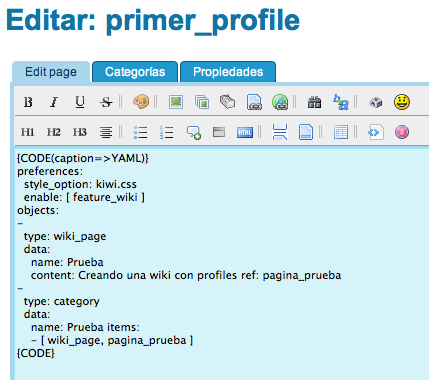
\includegraphics{../graphics/fig_editar_primer_profile.png}
\caption{Escribimos el contenido del \profile{} en una página wiki.}\label{fig:editar_primer_profile}
\end{figure}

\begin{figure}
\centering

\includegraphics{../graphics/fig_interfaz_plugin_data_channel.png}
\caption{Interfaz gráfica generada por el \textit{plug-in} \textit{Data Channel}, podemos ejecutar el \profile{} cómodamente con un clic de ratón.}\label{fig:interfaz_plugin_data_channel}
\end{figure}

\section{Implementación interna de los Profiles}

A continuación, para todas aquellas personas que estén interesadas en desarrollar y/o mejorar un \textit{Handler} o simplemente desean saber más sobre como funciona internamente la plataforma, se dará una explicación de las partes más interesantes que hacen posible que los \profiles{} existan tal y como los conocemos. Para ello, se explicará como se desarrolló el \textit{Users Handler} (el que se encarga de crear usuarios) por ser éste bastante sencillo de entender y que fue creado por el autor del \pfc{}. Aconsejamos al lector leer (si no se ha realizado anteriormente) el \appendixref{apendice-c} para obtener primero una visión complementaria de como está estructurado el código de \tiki{}. Sin más dilaciones, comenzamos.

\subsection{¿Cómo funciona por dentro un Handler?}

El código fuente que da vida a los \profiles{} se halla en la carpeta \code{lib/profilelib}. Dentro de dicho directorio nos encontramos con cuatro archivos importantes:

\begin{itemize}
    \item \code{profilelib.php}: Esta librería es la que da el funcionamiento principal de todo el código y la encargada de interpretar los documentos en formato \yaml{}, de buscar referencias de objetos en el propio \profile{}, de devolver un mensaje de error al usuario si algo ha ido mal, y de realizar las peticiones a otras plataformas \textit{wiki} si el \profile{} está alojado en otros repositorios. Normalmente el código que hay aquí no hace falta tocarlo para poder crear un \textit{Handler} a no ser que queramos añadir una nueva forma de interpretar los documentos (por ejemplo: que en lugar de leerlos en formato \yaml{} los hiciese en formato \json{}).

\item \code{channellib.php}: Esta librería es la que lleva el manejo de los \textit{Data Channels}, algunas tareas que realiza es la comprobación de que un \textit{Data Channel} puede ser ejecutado por un usuario, y otra es cargar en la interfaz los Channels que hay guardados en la base de datos. De manera idéntica a lo que se dijo en el punto anterior, no debemos modificar nada de este fichero.

\item \code{listlib.php}: Esta librería es la encargada de realizar peticiones a otros servidores y generar una base de datos con los \profiles{} que hay existentes en dicho repositorio.

\item \code{installlib.php}: Esta librería es la encargada de crear los dieciocho \textit{Handlers} que hay actualmente. Hay una clase principal denominada \code{Tiki\_Profile\_InstallHandler} y es sobre la que deberemos heredar si queremos crear un nuevo \textit{Handler}. Dicha clase determina los siguientes métodos: \code{\_\_construct()}, \code{canInstall()}, \code{install()}, \code{replaceReferences()} y \code{\_install()} y son importantes puesto que las clases que implementemos tendrán que sobre-escribirlos (dependiendo de las necesidades del \textit{Handler}). El nombre de la clase utilizado para el \textit{User Handler} es \code{Tiki\_Profile\_InstallHandler\_User} y hereda de \code{Tiki\_Profile\_InstallHandler}, los métodos que implementa son los siguientes:
\begin{itemize}
\item \code{getData()}: Este método lo que realiza es obtener la información del \profile{} (todo lo que le corresponde al \textit{Handler} de usuarios) y reemplazar las referencias que haya.
\item \code{canInstall()}: Este método se encarga de preguntar si se puede instalar el \profile{} o no y para ello comprueba que hay algo escrito dentro del \profile{}.
\item \code{\_install()}: Este es el método más importante ya que es el que realiza el grueso de la operación de añadir usuarios. Lo que hace es comprobar si están los campos que necesita el \textit{Handler} para funcionar y si es así llama a la librería \code{userlib.php} que es la encargada de crear nuevos usuarios.
\end{itemize}
En la \figureref{user-handler-impl} se muestra la implementación completa (por ser bastante breve) del \textit{User Handler}.
\end{itemize}

\begin{figure}
\begin{pyglist}[language=php]
  <?php
  class Tiki_Profile_InstallHandler_User extends Tiki_Profile_InstallHandler
  {
    function getData()
    {
      if( $this->data )
        return $this->data;
      $data = $this->obj->getData();
      $this->replaceReferences($data);

      return $this->data = $data;
    }

    function canInstall()
    {
      $data = $this->getData();
		
      if (isset($data)) return true;
      else return false;
    }
	
    function _install()
    {
      if ($this->canInstall())
      {
        global $userlib; if (!$userlib) require_once 'lib/userslib.php';

        $user = $this->getData();
				
        if (!$userlib->user_exists($user['name'])) {
          $pass = isset($user['pass']) ? $user['pass'] : $user['name'];
          $email = isset($user['email']) ? $user['email'] : '';
          if (isset($user['change']) && $user['change'] === false) {
            $userlib->add_user($user['name'], $pass, $email);
          } else {
            $userlib->add_user($user['name'], $pass, $email, $pass, true);
          }
        }

        if (isset($user['groups'])) {
          foreach ($user['groups'] as $group) {
            $userlib->assign_user_to_group($user['name'], $group);
          }
        }
				
        return $userlib->get_user_id($user['name']);
       }
    }
  }
\end{pyglist}
\caption{Implementación del \code{Users Handler}.}
\label{fig:user-handler-impl}
\end{figure}

      \chapter{Gestión dinámica de la plataforma \textsc{alma}} 
\label{chapter:gestion-dinamica}

\begin{center}
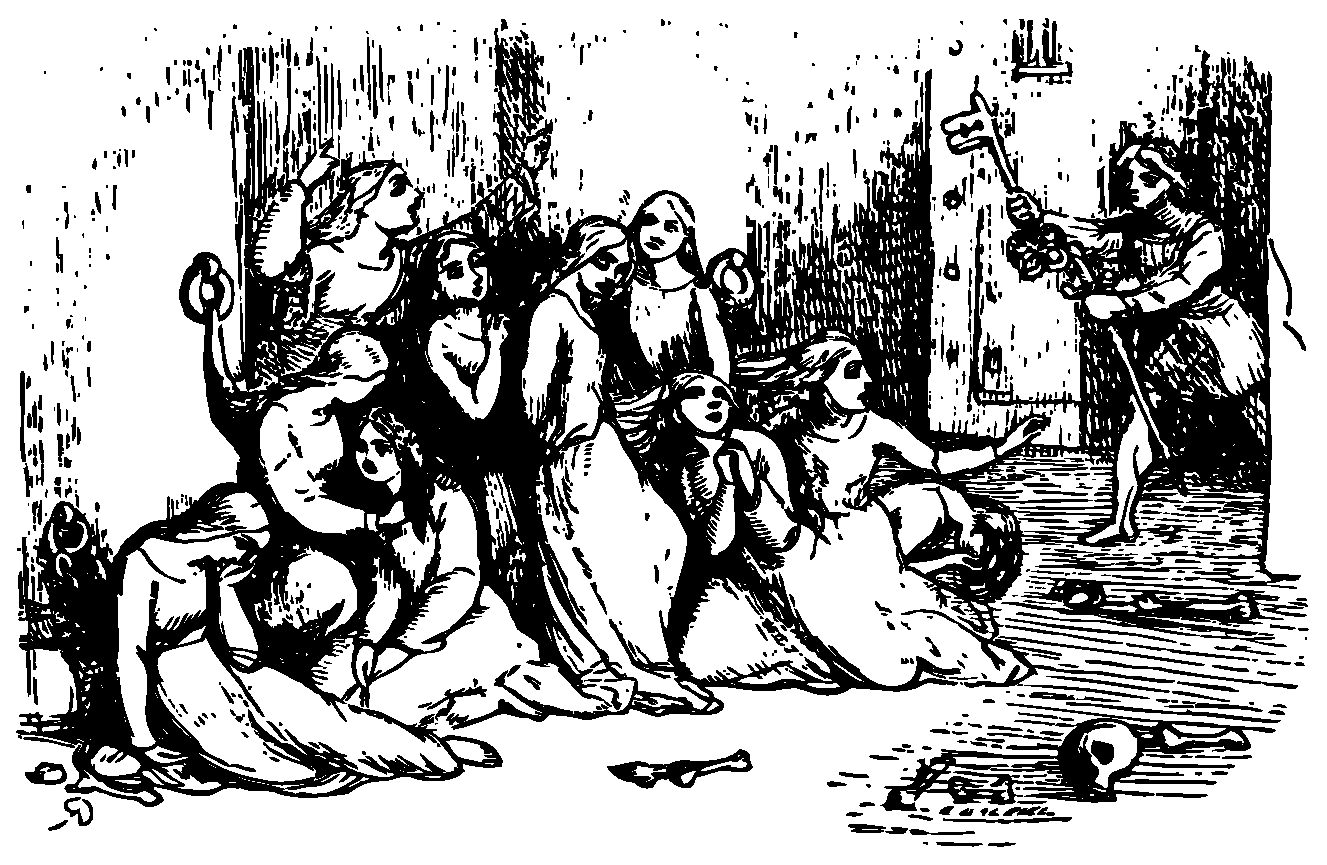
\includegraphics[scale=0.4]{../graphics/johnny_automatic_Jack_freeth_the_captives.eps}
\end{center}

\lettrine{E}{n este capítulo}, dividido en dos partes fundamentales, se mostrará en la primera que mejoras se han producido utilizando los \profiles{} (y desde el punto de vista de un administrador) en la creación de nuevas comunidades de práctica. En la segunda parte se mostrarán detalles internos de los \profiles{} realizados (no obstante, para analizar las implementaciones completas de dichos \profiles{} se deberá visitar el \appendixref{apendice-b}, ya que, en este capítulo sólo se enseñarán los fragmentos que se consideran relevantes).

\section{¿Qué ha cambiado en la gestión de \tiki{} utilizando Profiles?}

\subsection{¿Cómo se crea una nueva asignatura?}

En esta nueva situación, crear asignaturas (comunidades de práctica) se ha convertido en una tarea muy simple (cuando antes no lo era). Los pasos que tiene que seguir el administrador o docente para crear una nueva asignatura son los siguientes (se asume que ya están instalados los \profiles{} diseñados para \alma{} correctamente, en el \appendixref{apendice-c} se encuentra el manual de usuario que explica como hacerlo de manera muy detallada):

\begin{enumerate}
\item El administrador o docente ha de listar todas las páginas \textit{wiki} que están disponibles en \tiki{} (\figureref{listar_paginas_wiki_profiles}). Ha de buscar una llamada: \texttt{Crear\_Comunidad\_de\_Practica\_GUI}, en ella se encuentra la interfaz por la cuál se puede ejecutar el \profile{} que se encuentra definido en otra página \textit{wiki} denominada: \texttt{Crear\_Comunidad\_de\_Practica\_Template}.

\begin{figure}
\centering
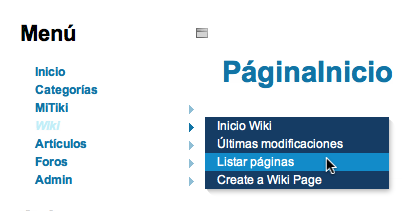
\includegraphics{../graphics/fig_listar_paginas_wiki_profiles.png}
\caption{Dado que el \profile{} es una página \textit{wiki} hay que buscar donde se encuentra éste.}\label{fig:listar_paginas_wiki_profiles}
\end{figure}

\item Una vez en la página \texttt{Crear\_Comunidad\_de\_Practica\_GUI} se escribe el nombre de la asignatura que se desee crear (\figureref{crear_asignatura_matematicas_profile}).

\begin{figure}
\centering
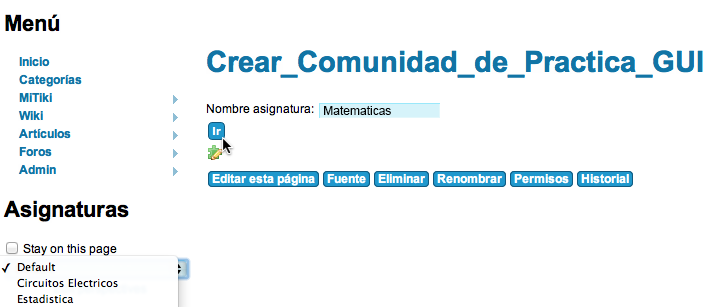
\includegraphics[width=\linewidth]{../graphics/fig_crear_asignatura_matematicas_profile.png}
\caption{Es tan sencillo como poner el nombre de la asignatura a crear y darle a Ir. El \profile{} se encargará del resto.}\label{fig:crear_asignatura_matematicas_profile}
\end{figure}

\item ¡Y listo, comunidad de práctica creada! A partir de ahora el administrador o docente deberá ir a la sección de usuarios y decidir quién quiere que sea miembro de dicha comunidad (\figureref{ejemplo_admin_usuarios}).
\end{enumerate}

\begin{figure}
\centering
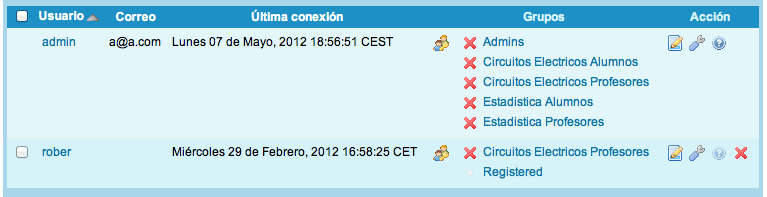
\includegraphics[width=\linewidth]{../graphics/fig_ejemplo_admin_usuarios.png}
\caption{En el panel de usuarios se pueden agregar qué usuarios pertenecen a qué grupos. Por defecto, por cada comunidad de práctica que se crea, el usuario \textit{admin} pertenece a cada grupo de dicha comunidad.}\label{fig:ejemplo_admin_usuarios}
\end{figure}

\section{Implementación interna de los \profiles{} desarrollados}

\subsection{Profile que configura \tiki{} a las necesidades de \alma{}}

\subsubsection{Objetivo}

El objetivo principal de este \profile{} es configurar una nueva instalación de \tiki{} y modificarla a las necesidades del proyecto \alma{}. Esto presenta múltiples ventajas, entre ellas: 

\begin{itemize}
\item Nos permite replicar \alma{} de una manera muy rápida y cómoda para un administrador. Si, por ejemplo, la instalación que existe actualmente sobre \tiki{} desapareciese (por el motivo que fuere), se podría descargar de nuevo el programa, ejecutar dicho \profile{} y tener una réplica exacta de la anterior \alma{} en ajustes y preferencias. De esta manera el administrador de la plataforma sólo se tiene que preocupar por recuperar los datos que se hayan guardado en la anterior instalación e importarlos en la nueva. 

\item Como punto que parte del anterior, nos sirve también para crear una réplica de \alma{} para hacer nuestras pruebas internas sin afectar al servidor principal, es decir, como plataforma de desarrollo. Este es el método que ha usado el autor del \pfc{} para crear los demás \profiles{}.
\end{itemize}

\subsubsection{¿Cómo se ha implementado?}

La lógica que se ha utilizado para crear este \profile{} es la que sigue en la \figureref{configuracion_alma_profile}. A continuación, se explican las etapas una a una:

\begin{figure}
\centering
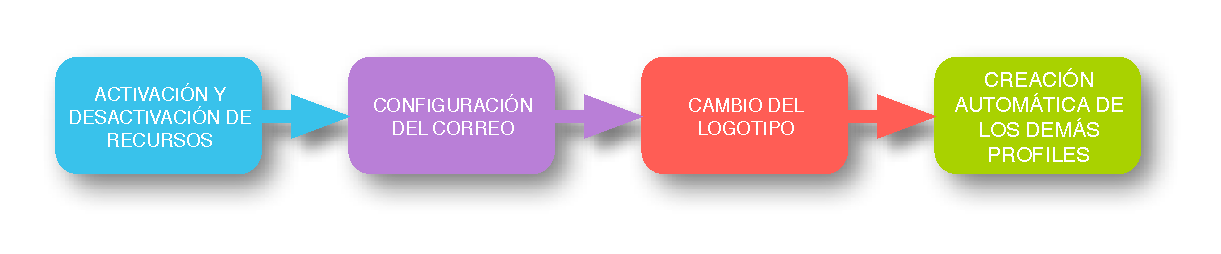
\includegraphics[width=\linewidth]{../graphics/fig_configuracion_alma_profile.eps}
\caption{Etapas empleadas para elaborar el \profile{} que configura \tiki{} a las necesidades de \alma{}.}\label{fig:configuracion_alma_profile}
\end{figure}

\begin{itemize}
\item \textit{Activación y desactivación de recursos}: Dado que \alma{} tiene unas necesidades muy concretas se han habilitado todos los elementos que hacen posible que funcionen las comunidades de práctica (entre ellos se activan los \profiles{}, las categorías y las perspectivas):

\begin{pyglist}[language=text]
  feature_categories:  y
  feature_mytiki: y
  feature_userPreferences: y
  feature_profiles: y
  feature_perspective: y
\end{pyglist}

Así mismo se desactivan múltiples características de \tiki{} que, en principio, no se van a utilizar (al menos por ahora). Si analizamos el \profile{}, encontraremos que se anulan los siguientes elementos: 

\begin{pyglist}[language=text]
  feature_blogs:  n  
  feature_file_galleries:  n
  feature_forums:  n
  feature_freetags:  n
  feature_help:  n
  feature_trackers: n
\end{pyglist}

\item \textit{Configuración del correo electrónico}: Se dan los datos necesarios para que se puedan enviar correos electrónicos desde la propia plataforma, ya sea para notificar a los usuarios de que se han registrado en una comunidad de práctica así como para recibir la contraseña en caso de extravío.

\begin{pyglist}[language=text]
  sender_email: alma@uah.es
  zend_mail_handler: smtp
  default_mail_charset: utf-8
  zend_mail_smtp_user: alma.disciplinar@gmail.com
  zend_mail_smtp_pass: password
  zend_mail_smtp_port: 465
  zend_mail_smtp_security: ssl
  zend_mail_smtp_auth: plain
  zend_mail_smtp_server: smtp.gmail.com
\end{pyglist}

\item \textit{Cambio del logotipo}: Se personaliza la imagen de \tiki{} sustituyendo el logotipo que trae por defecto a uno diseñado específicamente para \alma{}.

\begin{pyglist}[language=text]
  sitelogo_title: ALMA (Aula Libre Multidisciplinar Abierta)
  sitelogo_src: img/tiki/tikisitelogo.png
  sitelogo_alt: Alma
\end{pyglist}


\item \textit{Creación automática de los demás \profiles{}}: Por último se encarga de crear un grupo denominado \texttt{Profiles} donde se almacenarán los dos \profiles{} que se utilizan para crear comunidades de práctica (el \profile{} en si y su \textit{Data Channel} asociado).

\begin{pyglist}[language=text]
  objects:
    -
      type: wiki_page
      ref: wiki1
      data:
        name: Crear_Comunidad_de_Practica_GUI
        content: "{DATACHANNEL(channel=crear_comunidad)}
        nombre_asignatura, Nombre de la comunidad de practica
        {DATACHANNEL}"
    -
      type: wiki_page
      ref: wiki2
      data:
        name: Crear_Comunidad_de_Practica_Template
    -
      type: category
      ref: profilecateg
      data:
        name: Profiles
        items:
         - [ wiki_page, $wiki1 ]
         - [ wiki_page, $wiki2 ]
\end{pyglist}

Y se le asignan permisos específicos para que sólo los administradores puedan ver, editar y borrar todos los elementos que contenga dicha categoría.

\begin{pyglist}[language=text]
  permissions:
   Admins:
    objects:
     -
      type: category
      id: $profilecateg
      allow:
        - admin
\end{pyglist}

También se realizan los ajustes pertinentes (que no puedan ver, ni editar, ni borrar) para los demás grupos (\texttt{Registered}, \texttt{Anonymous}).

\begin{pyglist}[language=text]
   Registered:
    objects:
     -
      type: category
      id: $profilecateg
      deny: view, edit, view_category, edit_category
\end{pyglist}

\item \textit{Miscelánea}: Otros cambios que se realizan son las mejoras en los editores \wysiwyg{} (se añade la posibilidad de que los usuarios puedan crear fórmulas matemáticas) o se pone el lenguaje de \tiki{} en castellano.
 
 \begin{pyglist}[language=text]  
  language: es
  feature_wysiwyg:  y
  wysiwyg_default: y
  wysiwyg_optional: y
  wikiplugin_equation: y
  wikiplugininline_equation: y
\end{pyglist}

\end{itemize}

Si queremos analizar la implementación completa hay que visitar la \sectionnopageref{configuracion_alma} del \appendixref{apendice-b}.

\subsection{Profile que crea de manera automática comunidades de práctica} 

\subsubsection{Objetivo}

El objetivo de este conjunto de \profiles{} (se necesitan dos para llevar a cabo la tarea, aunque, el grueso de la operación realmente se produce en uno y el otro sirve como apoyo) está bastante claro. Por definición expresa, es el que simplifica la gestión de \tiki{} y son los que dan sentido completo a este \pfc{}.

\subsubsection{¿Cómo se ha implementado?}

Anteriormente se explicó como un administrador o docente podía crear una asignatura visitando la página \textit{wiki}: \texttt{Crear\_Comunidad\_de\_Practica\_GUI}. En la \figureref{esquema_flujo_profiles_interno} podemos ver como es realmente el flujo por detrás (la implementación que existe).

\begin{figure}
\centering
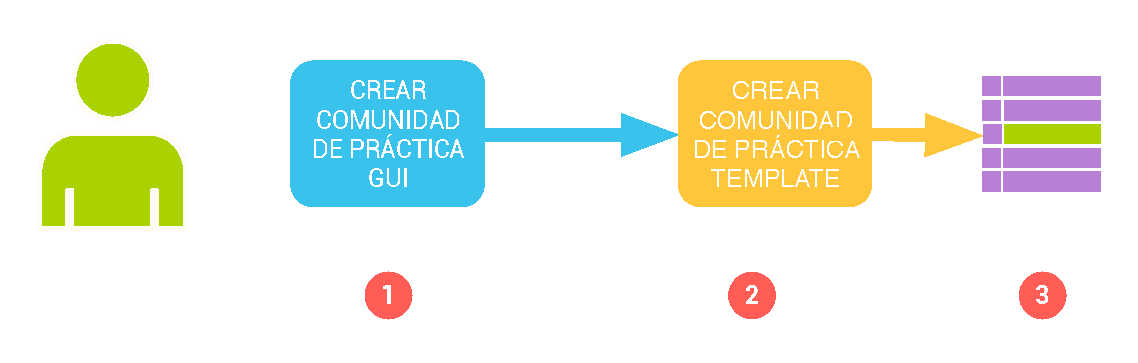
\includegraphics[width=\linewidth]{../graphics/fig_esquema_flujo_profiles_interno.eps}
\caption{Supongamos que un administrador o docente desea crear una asignatura. Para ello se dirige a la página \texttt{Crear\_Comunidad\_de\_Practica\_GUI}. Ésta es la encargada de dibujar la interfaz gráfica que es lo que el usuario ve como un campo para introducir un texto (aunque puede ser tan compleja como deseemos). Una vez que el administrador ha decidido el nombre de la asignatura y pulsa el botón enviar, la petición es enviada a la página \textit{wiki} \texttt{Crear\_Comunidad\_de\_Practica\_Template} que es donde se encuentran las instrucciones precisas para generar una comunidad de práctica. A continuación, se rellenan las variables oportunas para personalizar los nombres de los grupos, las páginas \textit{wikis}, etc y se ejecuta uno a uno las instrucciones que hay dentro de dicho \profile{} (tal y como explicamos en el capítulo anterior).}\label{fig:esquema_flujo_profiles_interno}
\end{figure}

Por defecto, los elementos que el \profile{} \texttt{Crear\_Comunidad\_de\_Practica\_Template} generan son los siguientes (podemos verlo de manera gráfica en la \figureref{explicacion_profile_comunidad}):

\begin{figure}
\centering
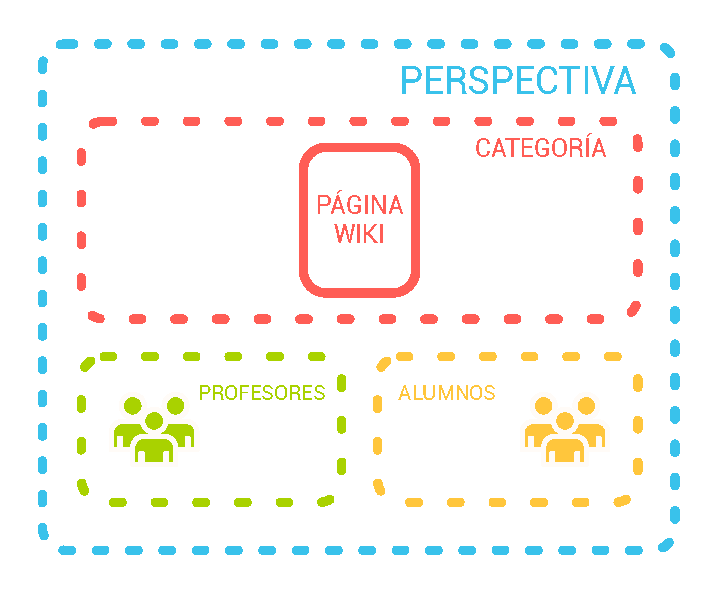
\includegraphics[width=.8\linewidth]{../graphics/fig_explicacion_profile_comunidad.eps}
\caption{Elementos que genera el \profile{} \texttt{Crear\_Comunidad\_de\_Practica\_Template}.}\label{fig:explicacion_profile_comunidad}
\end{figure}

\begin{itemize}
\item Se crea, por defecto, una página \textit{wiki} de bienvenida a la asignatura. Sirve como un punto de paso para cualquier miembro de la comunidad de práctica. Los posibles usos que se le pueden dar son variados, por ejemplo: se podría crear un listado de enlaces con las últimas novedades que han sucedido en la comunidad.

\begin{pyglist}[language=text]
  type: wiki_page
    ref: dashboard
    data:
     name: $profilerequest:nombre_asignatura$Asignatura sin nombre$ Homepage
     content: ”Bienvenido a tu nueva asignatura”
\end{pyglist}

\item Se crea una categoría que sirve para agrupar todos los elementos que se generen durante la actividad de la propia comunidad. Se utiliza por dos razones principalmente: la primera que así controlamos los permisos de dicha comunidad y sabemos, invariablemente, que sólo los miembros pueden actuar sobre los recursos que contiene; la segunda, los recursos quedan categorizados y facilitan la navegación y el orden dentro de \tiki{}.

\begin{pyglist}[language=text]
  objects: -
     type: category
     id: $project_root
     allow:
       - view
       - edit
       - wiki_view_history
       - wiki_view_source
       - minor
       - upload_picture
       - rollback
       - view_category
       - search
       - delete_account
       - group_view
       - group_view_members
       - add_object
       - modify_object_categories
\end{pyglist}

\item Se generan dos grupos: \textit{Profesores} y \textit{Alumnos} de dicha comunidad. Cada uno tienen unos permisos detallados, por ejemplo: los alumnos no pueden borrar las ediciones que hayan realizado en una página \textit{wiki} mientras que los profesores sí. Si un usuario no pertenece a ninguno de estos dos grupos (sea la comunidad de práctica que sea) se considera que no es miembro de ésta y por lo tanto no aparece la asignatura en el menú \textit{Asignaturas}.

\item Se crea una perspectiva que es la encargada de realizar el \q{cambio de contexto} de una comunidad de práctica a otra.

\begin{pyglist}[language=text]
  type: perspective
    ref: perspective
    data:
     name: $profilerequest:nombre_asignatura$sin nombre$
     preferences:
      category_jail: $project_root
      wikiHomePage: $dashboard
      browsertitle: $profilerequest:nombre_asignatura$Asignatura sin nombre$
      style: fivealive.css
      style_option: kiwi.css
      feature_wysiwyg: y
      wysiwyg_default: y
      wysiwyg_optional: y
\end{pyglist}

\item Por último se ajustan todos los permisos de manera adecuada por cada elemento creado anteriormente.

\begin{pyglist}[language=text]
  permissions:
   Member:
    autojoin: y
    allow:
        - view
        - edit
        - wiki_view_history
        - wiki_view_source
        - minor
        - upload_picture
        - rollback
        - view_category
        - search
\end{pyglist}
\end{itemize}

La implementación completa, tanto del \profile{} \texttt{Crear\_Comunidad\_de\_Practica\_Template} como del \texttt{Crear\_Comunidad\_de\_Practica\_GUI}, la podemos encontrar en la \sectionref{creacion-comunidad} y \sectionref{creacion-comunidad-gui}, respectivamente, del \appendixref{apendice-b}.
    
    \part{Sumario}
      \chapter{Conclusiones} 
\label{chapter:conclusiones}

\begin{center}
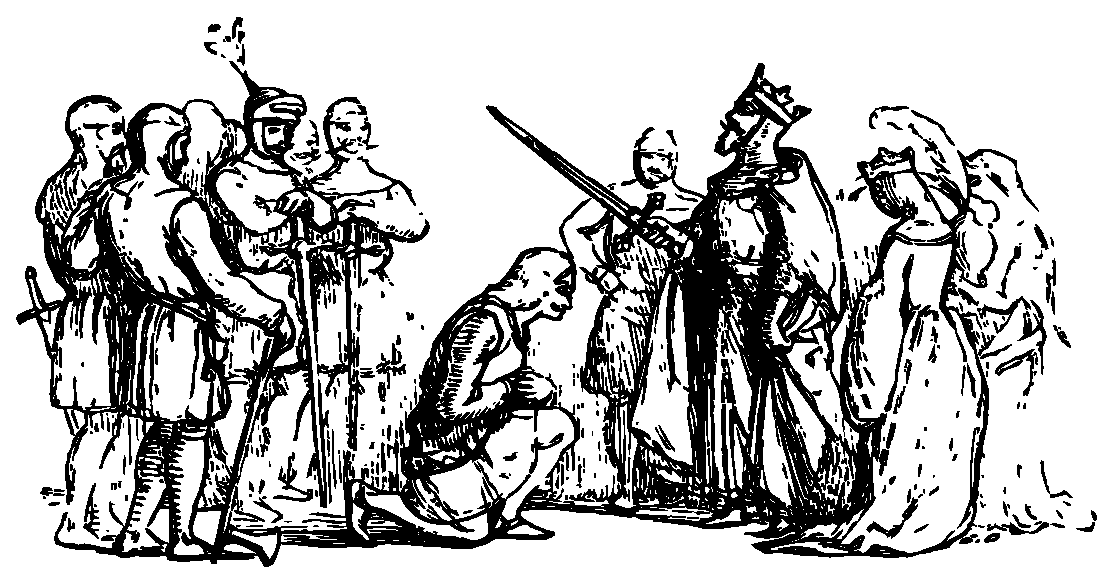
\includegraphics[scale=0.4]{../graphics/johnny_automatic_Jack_and_King_Arthur.eps}
\end{center}

\section{Conclusiones de la implementación}

Implementar las comunidades de práctica con \tiki{} fue una decisión muy importante que tuvimos que sopesar bastante. Sobre todo, cuando estábamos trabajando con un conjunto grande de usuarios y su gestión se tornaba de vital importancia para el éxito del proyecto. Los \profiles{} han resultado ser una herramienta muy útil que ayuda a gestionar la plataforma de una manera bastante cómoda. Entre las alternativas que podemos encontrar en el mercado, no existe un concepto similar y que ofrezca tantas posibilidades como lo hacen éstos en \tiki{}.

Si hay algo que es importante a tener en cuenta es, que las nuevas tecnologías deben ir siempre un paso por delante y tienen que promover, por encima de todas las cosas, la facilidad de uso. Hay muchos colectivos que no están tan implicados, al menos no de una manera tan profunda, con las nuevas tecnologías y son a ellos a los que más hay que tener presente cuando se piensa en crear una nueva interfaz de usuario. Es evidente que \tiki{} tiene que mejorar en múltiples aspectos, sobre todo en la facilidad de uso. También lo tiene que hacer en la propia herramienta de los \profiles{}, puesto que, aún se tiene que aprender a utilizar \yaml{} y eso es algo que no está al alcance de todo el mundo. 

Las conclusiones positivas que se extraen de este trabajo realizado son varias:

\begin{itemize}
\item Se ha conseguido implementar el proyecto \alma{} con bastante éxito y tal cual se pedía en los requisitos. Prueba de ello es que se está utilizando de manera real con un grupo de usuarios considerable en algunas asignaturas impartidas en la \textsc{uah} (en la \figureref{demostracion_alma} se puede ver una captura).
\item Se han mejorado considerablemente las tareas administrativas por parte de un administrador respecto a la que ofrecía originalmente el flujo de trabajo sin \profiles{}. Y esa mejora repercute en una cosa: \textit{productividad}.
\item Estamos contentos de haberlo implementado en \tiki{} (pese a que no es el \textit{software} perfecto, ahora veremos porqué), ya que, esta herramienta, aúna a la vez simplicidad y complejidad. Simplicidad porque es un programa que nada más instalarlo, se puede usar sin mayor complicación. Complejidad porque como hemos visto, se ha comportado de manera excelente a la hora de buscar \q{casos de uso} más complejos.
\end{itemize}

\begin{figure}
\centering

\includegraphics[width=\linewidth]{../graphics/fig_demostracion_alma.png}
\caption{Implementación real de \textsc{alma} con \tiki{}.}\label{fig:demostracion_alma}
\end{figure}

Por contra, en los aspectos negativos nos encontramos que:

\begin{itemize}
\item Uno de los requisitos que pedíamos cuando estábamos buscando un \textit{software} para implementar las comunidades de práctica era: \textit{la instalación y el manejo de la plataforma debe de ser sencillo}. Este hecho, nos limitó un poco el campo de búsqueda de aplicaciones que pudieran crear, hipotéticamente, un gran colectivo de usuarios trabajando con las comunidades de práctica. Todas las aplicaciones que analizamos están basadas en \php{} por ser, precisamente, uno de los lenguajes más fáciles de aprender y de instalar en un servidor. Pero, hay otras plataformas programadas en otros lenguajes de programación como \textsc{java} y que son bastante más potentes que las que hay en \php. Entre muchas propuestas nos encontramos a  \textit{Liferay} \cite{web:liferay} o \textit{Alfresco} \cite{web:alfresco} y que se utilizan, sobre todo, en entornos empresariales. Éstos \cms{} tienen una muy buena implementación del concepto de grupos y recursos y una interfaz de usuario bastante más amigable que la que ofrece \tiki{}. Quizá, implementar las comunidades de práctica en esas plataformas hubiera sido más sencillo que hacerlo en \tiki{} (aún sin contar con los \profiles{}), pero, eso si, aumentando considerablemente la dificultad de modificación del código fuente en dichas aplicaciones (requieren tener un buen conocimiento interno de su estructura, que es infinitamente más compleja que la que utiliza \tiki{}).

\item La herramienta de los \profiles{} aún está en construcción y, debido a esto, las especificaciones de los \textit{Handlers} cambian con bastante frecuencia (aunque cada vez menos). Actualmente se están centrando en mejorar la experiencia de usuario para permitir que cualquier persona pueda usarlos y lo haga sin mucho esfuerzo. Quizá, si hubiéramos esperado más tiempo a la hora de ejecutar este proyecto, es bastante posible que la creación de los \profiles{} se hubiera realizado a \textit{golpe de ratón} en lugar de a \textit{golpe de \yaml{}}.

\end{itemize}

\section{Lecciones aprendidas}

Este \pfc{} ha tenido una duración aproximada de unos dos años (desde que se comenzó a plantear la idea hasta que se ha definió el objetivo concreto), y durante ese tiempo han sucedido múltiples eventos que han servido al autor para aprender en muchos ámbitos. Una de las mayores noticias fue la aceptación por parte de Google para participar en su programa \textit{Summer of Code} de 2009 en la mejora de los \textit{Workspaces} (que no es un concepto bastante parecido al de las comunidades de práctica) de \tiki{}. Entre otras cosas se aprendió:

\begin{itemize}

\item Como se organiza una plataforma de código abierto (su arquitectura interna) y como los recursos humanos son coordinados para la consecución de un objetivo común.

\item A mejorar las habilidades codificando con \php{}. Al comenzar el proyecto desconocía cómo se programaba en este lenguaje y, al acabarlo, puedo decir orgulloso que es uno de los que más conozco.

\item A mejorar mi nivel de inglés. Estar en un ambiente de índole internacional me permitió conocer nueva gente y a expresar mis ideas dando charlas en público.

\item A aprender el maravilloso mundo de la tipografía y la maquetación. Maquetar un libro es una tarea que no es trivial y que requiere un esfuerzo y unas ganas por aprender bastante importantes. El resultado que has podido ver (y leer), es fruto de todo este esfuerzo.

\end{itemize}

\section{Futuras lineas de trabajo}

Hay que reconocer que, aunque durante todo este \pfc{} se han estado ensalzando las virtudes de \tiki{}, éste posee unas serie de desventajas considerables en cuanto a varios aspectos de la plataforma. La verdad sea dicha, hay bastantes cosas que se pueden enriquecer aún más y que son susceptibles de que alguien coja el testigo y las convierta en realidad, entre ellas destacamos (sin ningún orden concreto de prioridad):

\begin{enumerate}

\item Mejorar las interfaces gráficas de administración de \profiles{} de \tiki{}. Actualmente los \profiles{} requieren que una persona tenga ciertos conocimientos técnicos a la hora de poder implementarlos. Eso en un entorno docente puede ser que no sea factible, quizá un profesor está al cargo de alguna asignatura y por el mero hecho de que ni si quiera sabe qué es \yaml{} no debería ser discriminado. ¿De qué manera podríamos solucionar este problema? Actualmente Apple \cite{web:apple} en su sistema operativo \textsc{os x} \cite{web:apple-os-x} tiene una herramienta llamada \textit{Automator} \cite{web:apple-automator} que enmascara a un usuario que no sabe de programación la tarea de crear pequeños programas que hagan ciertas tareas (conocidos como \textit{flujos de trabajo}). Para crear un nuevo programa el usuario simplemente tiene que ir arrastrando pequeños componentes que realizan una acción concreta (por ejemplo, \q{listar todos los documentos en un directorio}) e ir uniendo más componentes al flujo (podría añadir: \q{seleccionar aquellos ficheros que tengan formato \textsc{pdf}}) hasta que obtiene un programa que realiza una tarea concreta (podría finalizar el flujo añadiendo: \q{y mover dichos archivos a la carpeta de mis documentos}). En la \figureref{flujo_trabajo_automator} podemos ver el flujo real que se ha comentado antes. En \tiki{} se podría realizar algo similar con los \profiles{} y eso es algo que una persona que no tiene muchos conocimientos técnicos, puede asumirlo y aprender a usarlo.

\item Los \profiles{} que se han creado son muy \q{rígidos}, y asumen muchas cosas por defecto (por ejemplo sólo crea una \textit{wiki}, pero no crea un foro). Se podrían crear más \profiles{} que abarquen más casos de uso.

\item El sistema de los \textit{Data Channels} no tiene una implementación muy clara. Sería útil crear un apartado en \tiki{} donde se pudieran guardar los \textit{Data Channels} creados al igual como se listan los recursos en las categorías. Esto permitiría mejorar la facilidad de uso de la plataforma.

\item Enriquecer y adaptar la documentación que se encuentra en: \url{http://doc.tiki.org}. Muchas veces cuando un usuario necesita saber cosas concretas de la plataforma tiene que acudir a la documentación oficial para aclarar sus dudas. El problema es que en muchas áreas ésta no está de forma clara o incluso contiene información anticuada de anteriores versiones que ya no es vigente y que no sirve. Mejorar la documentación ayudaría a que los usuarios tuviesen un mejor conocimiento de la plataforma.

\item La traducción al castellano del propio \tiki{} es irregular y, en ocasiones, de mala calidad: se entremezclan oraciones en inglés con algunas en castellano. De cara a mostrar una buena imagen, se debería traducir de forma correcta.
\end{enumerate}

\begin{figure}
\centering
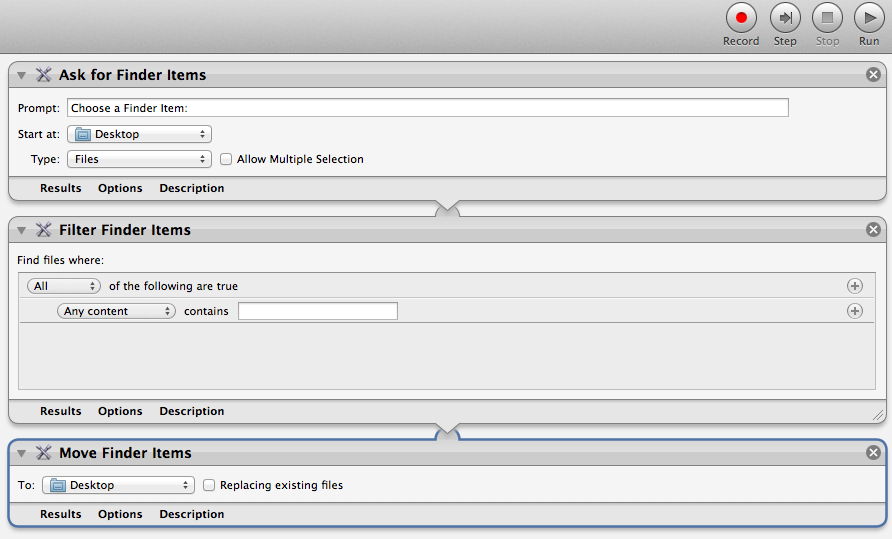
\includegraphics[width=\linewidth]{../graphics/fig_flujo_trabajo_automator.png}
\caption{Ejemplo del programa Automator.}\label{fig:flujo_trabajo_automator}
\end{figure}

    \addcontentsline{toc}{part}{\appendixtocname}
    \appendixpage*

     \begin{appendices}
       \chapter{YAML}
\label{appendix:yaml}

\glsreset{yaml}

\section{¿Qué es YAML?}

\yaml{} es un formato de serialización de datos creado por Clark Evans, Ingy döt Net y Oren Ben-Kiki en 2001 y que está fuertemente inspirado en lenguajes como \xml{}, C, Python y Perl. A diferencia de \xml{}, la sintaxis de \yaml{} es muy liviana y es muy fácil de interpretar por las personas, de hecho, surgió como una alternativa a \xml{} por considerar a éste un poco \textit{engorroso} de crear documentos y, sobre todo, de leerlos.

Actualmente tiene una amplia aceptación en el mundo de la programación, donde, lenguajes tan populares y conocidos como son: C, Python, \textsc{java}, Ruby, Haskell, JavaScript (y otros tantos más) tienen implementaciones, en forma de librerías externas en algunos casos o incluidas en el propio lenguaje en otros, de un intérprete de \yaml{}. Los usos que se le pueden dar son tan variados que dependen del propio programador y lo que desee hacer con el formato aunque, generalmente, se suele utilizar para crear archivos de configuración que luego los programas pueden leer y modificar las preferencias del mismo; un ejemplo claro lo encontramos en el programa \textit{Jekyll} \cite{web:jekyll}. Éste es un generador de sitios web estáticos (muy popular entre la comunidad de programadores) y que utiliza \yaml{} para pasar datos básicos de configuración al propio programa (\figureref{ejemplo_yaml}).
Encontramos la misma situación en varios programas de renombre como: \textit{Ruby on Rails} \cite{web:ruby-on-rails} o \textit{Symfony} \cite{web:symfony} que son dos aplicaciones que sirven para crear páginas web dinámicas y que utilizan a \yaml{} con el mismo objetivo: configurar las propias aplicaciones.

\begin{figure}
\centering
\includegraphics[scale=0.8]{../graphics/fig_ejemplo_yaml.png}
\caption{Ejemplo de configuración del programa Jekyll utilizando \yaml{}.}\label{fig:ejemplo_yaml}
\end{figure}

El hecho de que los \profiles{} utilicen \yaml{} no es otro que por la claridad de lectura que se obtiene con ellos. Además, en el caso de \php{}, hay una implementación del formato incluida en el propio lenguaje que está bastante optimizada.

En la web podemos encontrar multitud de recursos para aprender sobre la especificación de \yaml{}. En este apéndice, en concreto, sólo se mostrarán los elementos más básicos del lenguaje. Si deseamos obtener más información no hay nada mejor que ir a la página oficial \cite{web:especificacion-yaml} donde siempre encontraremos la última versión de la especificación de \yaml{}.

\section{Especificación de YAML}

\yaml{} tiene dos consideraciones básicas previas que se deben cumplir si se quiere producir un documento que sea validado por un intérprete:

\begin{itemize}
\item El documento tiene que estar estructurado utilizando la \textit{indentación} con espacios en blanco, por contra no se permite el uso del tabulador para \textit{indentar}.

\item El documento debe de estar codificado en formato \textit{Unicode}, bien sea en \textsc{utf-8} o \textsc{utf-16}.
\end{itemize}

A continuación, vamos a ver los componentes básicos que conforman un documento en \yaml{} (y realmente, los \profiles{} utilizan la combinación de estos elementos sencillos):

\subsection{Comentarios}

\begin{pyglist}[language=yaml]
  # El símbolo almohadilla se utiliza como comentario.
  edad: 20 # Los comentarios se pueden situar donde queramos
\end{pyglist}

\subsection{Comienzo de documento}

\begin{pyglist}[language=yaml]
  --- # Tres guiones indican al intérprete que comienza un nuevo documento de YAML
  --- # Podemos tener tantos nuevos documentos como queramos en un mismo fichero
  --- # Los dos primeros documentos están vacíos, este en cambio, no
  edad: 24
\end{pyglist}

\subsection{Valores básicos}

\begin{pyglist}[language=yaml]
  ---
  nombre: Aldo # Un valor básico es como una variable
  edad: 20 # Se compone de una etiqueta : valor
\end{pyglist}

\subsection{Listas}

\begin{pyglist}[language=yaml]
  --- # Frutas (Formato largo)
  - Manzana # Conjunto de elementos que comparten algo
  - Pera # Entre el guión - y el nombre hay un espacio
  - Melón # En la linea siguiente comenzamos un nuevo documento de YAML
  
  --- # Frutas (Formato corto)
  [Manzana, Pera, Melón]  # Ambas notaciones son equivalentes
\end{pyglist}

\subsection{Arrays Asociativos}

\begin{pyglist}[language=yaml]
  # (Formato Largo) Se indentan, se muestran los espacios utilizados
  ---
     nombre: Aldo Borrero
     edad: 24

  --- # (Formato Corto) Se engloban en corchetes, no hay que indentar
   {nombre: Aldo Borrero, edad: 24}
\end{pyglist}

\subsection{Cadenas de caracteres}

\begin{pyglist}[language=yaml]
  --- # No hay que poner comillas a las cadenas
  string: Puedo poner lo que quiera sin comillas
\end{pyglist}

\subsection{Texto de múltiples lineas}

\begin{pyglist}[language=yaml]
  # Podemos tener textos que queramos preservar los retornos de linea

  --- |
   Esto es un ejemplo de un texto
   que tiene múltiples lineas.
       YAML preserva el texto
       de manera inteligente.
   ¡Como cabría esperar!
\end{pyglist}

\subsection{Texto de múltiples lineas convertido a una}

\begin{pyglist}[language=yaml]
  --- >
     Este texto aunque
     tiene múltiples
     lineas
     será convertida a una sola
\end{pyglist}

\subsection{Listas de arrays asociativos}

\begin{pyglist}[language=yaml]
  --- # Podemos crear estructuras más complejas utilizando las simples
  - {nombre: Aldo Borrero, edad: 24}
  - nombre: Michael Jackson
    edad: 50
\end{pyglist}

\subsection{Arrays asociativos de listas}

\begin{pyglist}[language=yaml]
  ---
  alumnos: [Pepito Pérez, Jose María Gonzalo]
  mujeres: [] # No hay ninguna mujer, array vacio
  perros:
    - Lassie
    - Milú
\end{pyglist}
       \chapter{Código Fuente} 
\label{appendix:apendice-b}

\section{Organización del código de \tiki{}}
\label{appendix:organizacion-codigo}

\tiki{} es un proyecto de código abierto que ha sido desarrollado completamente en \php{}. La organización del código sigue una distribución precisa y lógica. Aún así, para una persona neófita que se interna por primera vez en el desarrollo de alguna librería o modificación, puede pensar que la estructura del propio proyecto es algo caótica. A continuación, se muestra un listado de los directorios y archivos más importantes de \tiki{} así como una breve descripción de ellos:
 
\begin{itemize}
\item \textit{lib/}: Este directorio guarda todas las librerías principales de \tiki{}, si queremos realizar una modificación en el núcleo del programa este es nuestro sitio.

\item \textit{db/}: En este directorio se guardan las definiciones del esquema \textit{relacional} de \tiki{}. Aquí es donde se aloja el archivo \texttt{local.php}.

\item \textit{db/local.php}: Este archivo guarda la configuración a la base de datos que hayamos instalado en \tiki{}. Si queremos reinstalar todo desde cero, simplemente hay que limpiar la base de datos y borrar este archivo.

\item \textit{templates/}: Este directorio guarda las plantillas programadas en Smarty \cite{web:smarty}.

\item \textit{templates\_c/}: Este directorio sirve para guardar la \textit{caché} de \tiki{}. Normalmente no es útil cambiar nada de aquí (aunque se puede borrar el directorio para obligar a que \tiki{} regenere los datos de nuevo).

\item \textit{img}: Este directorio guarda la identidad de \tiki{}. Es útil por si se quiere cambiar el logotipo que muestra por defecto por uno propio.
\end{itemize}

\section{Listado de Profiles}

Se listan todos los \profiles{} que han sido diseñados para llevar a cabo este proyecto:

\subsection{Profile: Configuración de ALMA}
\label{section:configuracion_alma}

\begin{pyglist}[language=text]
Este profile configura Tikiwiki para trabajar en ALMA.

Crea también los \profiles{} necesarios para crear asignaturas de manera automática.

Se puede ejecutar directamente en Admin > Profiles > Advanced > Profile Tester

Esta sección se encarga de configurar las opciones generales de Tiki. ¡No olvides 
cambiar la contraseña del correo por la contraseña original!

Tampoco olvides copiar el contenido de Crear_Comunidad_de_Practica_Template 
a la página wiki con el mismo nombre!

{CODE(caption="YAML" wrap="1")}
preferences:
  language: es
  feature_wysiwyg:  y
  wysiwyg_default: y
  wysiwyg_optional: y
  wikiplugin_equation: y
  wikiplugin_perspective: n
  wikiplugininline_perspective: n
  wikiplugininline_equation: y
  feature_blogs:  n
  feature_categories:  y
  feature_file_galleries:  n
  feature_forums:  n
  feature_freetags:  n
  feature_help:  n
  feature_trackers:  n
  feature_mytiki:  y
  feature_userPreferences:  y
  feature_profiles: y
  feature_perspective: y
  allowRegister:  y
  min_username_length:  1
  max_username_length:  50
  min_pass_length:  4  
  forgotPass:  y
  cookie_name:  ALMA
  wikiHomePage:  HomePage
  sender_email:  alma@uah.es
  siteTitle:  ALMA
  browsertitle: ALMA
  site_title_location: before
  server_timezone: Madrid/Europe
  display_timezone: Madrid/Europe
  zend_mail_handler: smtp
  default_mail_charset: utf-8
  zend_mail_smtp_user: alma.disciplinar@gmail.com
  zend_mail_smtp_pass: password
  zend_mail_smtp_port: 465
  zend_mail_smtp_security: ssl
  zend_mail_smtp_auth: plain
  zend_mail_smtp_server: smtp.gmail.com
  log_mail: n
  wikiplugin_datachannel: y
  profile_channels: crear_comunidad, tiki://local, Crear_Comunidad_de_Practica_Template, Admins
  sitelogo_title: ALMA (Aula Libre Multidisciplinar Abierta)
  sitelogo_src: img/tiki/tikisitelogo.png
  sitelogo_alt: Alma
{CODE}

Esta sección se encarga de crear las páginas Wiki con el Profile de Crear 
Comunidad de Paractica y su Data Channel correspondiente. Los asigna al grupo 
de Profiles y sólo los admins son capaces de ejecutar y ver esas páginas.

{CODE(caption="YAML" wrap="1")}
objects:
  -
    type: wiki_page
    ref: wiki1
    data:
      name: Crear_Comunidad_de_Practica_GUI
      content: "{DATACHANNEL(channel=crear_comunidad)}nombre_asignatura, 
      Nombre de la comunidad de practica{DATACHANNEL}"
  -
    type: wiki_page
    ref: wiki2
    data:
      name: Crear_Comunidad_de_Practica_Template
      content: Rellenar el contenido de esta pagina con el archivo del mismo nombre
  -
    type: category
    ref: profilecateg
    data:
      name: Profiles
      description: Categoria donde se almacenan los profiles de las comunidades de practica
      items:
       - [ wiki_page, $wiki1 ]
       - [ wiki_page, $wiki2 ]
permissions:
 Admins:
  objects:
   -
    type: category
    id: $profilecateg
    allow:
      - admin
 Registered:
  objects:
   -
    type: category
    id: $profilecateg
    deny: view, edit, view_category, edit_category
 Anonymous:
  objects:
   -
    type: category
    id: $profilecateg
    deny: view, edit, view_category, edit_category
{CODE}

Creamos el menú que permite cambiar de asignatura a los usuarios que estén
registrados en la plataforma.

{CODE(caption="YAML", wrap="1")}
objects:
 -
  type: module
  ref: switcher
  data:
   name: perspective
   position: left
   order: 10
   groups: [ Registered ]
   params:
     title: Asignaturas
{CODE}
\end{pyglist}

\subsection{Profile: Creación Comunidad de Práctica}
\label{section:creacion-comunidad}

\begin{pyglist}[language=text]
!!!!!Creación de una asignatura usando Profiles

{CODE(caption=>YAML,wrap=1)}
mappings:
 Member: $profilerequest:nombre_asignatura$Asignatura sin nombre$ Alumnos
 Lead: $profilerequest:nombre_asignatura$Asignatura sin nombre$ Profesores
objects:
 -
  type: category
  ref: project_root
  data:
   name: $profilerequest:nombre_asignatura$Asignatura sin nombre$
   parent: 0
   items:
    - [ wiki page, $dashboard ]
 -
  type: perspective
  ref: perspective
  data:
   name: $profilerequest:nombre_asignatura$sin nombre$
   preferences:
    category_jail: $project_root
    wikiHomePage: $dashboard
    browsertitle: $profilerequest:nombre_asignatura$Asignatura sin nombre$
    style: fivealive.css
    style_option: kiwi.css
    feature_wysiwyg: y
    wysiwyg_default: y
    wysiwyg_optional: y
 -
  type: wiki_page
  ref: dashboard
  data:
   name: $profilerequest:nombre_asignatura$Asignatura sin nombre$ Homepage
   content: "Bienvenido a tu nueva asignatura"
permissions:
 Member:
  autojoin: y
  allow:
      - view 
      - edit
      - wiki_view_history
      - wiki_view_source
      - minor
      - upload_picture
      - rollback
      - view_category
      - search
      - delete_account
      - group_view
      - group_view_members
      - view_category
      - add_object
      - modify_object_categories
  objects:
   -
    type: category
    id: $project_root
    allow:
      - view 
      - edit
      - wiki_view_history
      - wiki_view_source
      - minor
      - upload_picture
      - rollback
      - view_category
      - search
      - delete_account
      - group_view
      - group_view_members
      - add_object
      - modify_object_categories
   -
    type: perspective
    id: $perspective
    allow: [ perspective_view ]
 Lead:
  autojoin: y
  allow:
      - view 
      - edit
      - wiki_view_history
      - wiki_view_source
      - minor
      - upload_picture
      - rollback
      - view_category
      - search
      - delete_account
      - group_view
      - group_view_members
      - view_category
      - add_object
      - modify_object_categories
      - remove
      - rollback
      - wiki_attach_files
      - admin_attachments
      - view_attachments
      - upload_picture
      - minor
      - rename
      - lock
      - edit_structures
      - edit_copyrights
      - wiki_view_comments
      - wiki_view_ratings
      - wiki_vote_ratings
      - wiki_admin_ratings
      - wiki_view_history
      - use_HTML
  objects:
   -
    type: category
    id: $project_root
    allow:
      - view 
      - edit
      - wiki_view_history
      - wiki_view_source
      - minor
      - upload_picture
      - rollback
      - view_category
      - search
      - delete_account
      - group_view
      - group_view_members
      - view_category
      - add_object
      - modify_object_categories
      - remove
      - rollback
      - wiki_attach_files
      - admin_attachments
      - view_attachments
      - upload_picture
      - minor
      - rename
      - lock
      - edit_structures
      - edit_copyrights
      - wiki_view_comments
      - wiki_view_ratings
      - wiki_vote_ratings
      - wiki_admin_ratings
      - wiki_view_history
      - use_HTML
   -
    type: perspective
    id: $perspective
    allow: [ perspective_view ]
{CODE}
\end{pyglist}

\subsection{Profile: Interfaz para Crear Comunidad de Practica}
\label{section:creacion-comunidad-gui}

\begin{pyglist}[language=text]
Este Profile genera una comunidad de práctica con el nombre que se le especifique:
{DATACHANNEL(channel=crear_comunidad)}
nombre_asignatura, Nombre asignatura
{DATACHANNEL}
\end{pyglist}
       \chapter{Manual de Usuario}
\label{appendix:apendice-c}

\section{Obtención del código fuente}

Todo el código que se ha producido para este \pfc{} se ha subido a un repositorio de \textit{BitBucket} \cite{web:bitbucket} (que es un servidor que permite alojar código fuente de manera gratuita y que utiliza el gestor de código distribuido \textit{Mercurial}, conocido también como: \texttt{hg} \cite{web:mercurial}).

Para descargar el código utilizando \texttt{hg} podemos ejecutar el siguiente comando en la terminal:

\begin{pyglist}[language=bash]
  $ hg clone https://bitbucket.org/aldoborrero/alma-profiles
\end{pyglist}

También podemos obtener una versión comprimida lista para descargar por \textit{http} si acudimos al siguiente enlace:

\begin{pyglist}[language=html]
https://bitbucket.org/aldoborrero/alma-profiles/get/v1.2.zip
\end{pyglist}

El directorio que obtendremos al descomprimir será el siguiente:

\begin{itemize}
\item \code{config.yml}: Este archivo contiene el \profile{} de configuración de \alma{}.
\item \code{Crear\_Comunidad\_de\_Practica\_GUI.yml}: Contiene el Data Channel.
\item \code{Crear\_Comunidad\_de\_Practica\_Template.yml}: Contiene la implementación del \profile{} que genera las comunidades de práctica.
\item \code{logo}: Este directorio en su interior posee el logotipo que utiliza \alma{}.
\item \code{mail}: Este directorio contiene una implementación alternativa de la librería de correo que utiliza \tiki{} y que soluciona ciertos problemas que teníamos con la antigua. Los ficheros que hay dentro son:

	\begin{itemize}
	\item \code{TikiMaillib.diff}: La nueva implementación de la librería de correo re-escrita por el autor del \pfc{}. Hay que decir que la implementación no es completa, sólo funciona para los requisitos que tiene \alma{} y no contempla otros casos de uso. Se desarrolló sólo con el objetivo de solucionar el problema que nos surgió, ¡no para reemplazar al original de manera completa!
	\item \code{swift}: Código fuente del proyecto \code{SwiftMailer} \cite{web:swiftmailer} que es una librería escrita en \php{} que permite trabajar con el envío de correos electrónicos de manera sencilla.
	\end{itemize}
\end{itemize}

\section{Requisitos previos}

Para poder ejecutar el código fuente se asume que el usuario ha instalado correctamente \tiki{} y que no ha configurado más que las opciones básicas de la instalación. También se asume que el usuario posee una versión de \code{UNIX}, da igual si es \code{Linux}, \code{OS X} o \code{BSD} (aunque los comandos se pueden adaptar fácilmente a un entorno \texttt{Windows}).

\section{Instalación}

El primer paso que se va a realizar es proceder a la sustitución de la librería de correo de \tiki{}, así pues, hay que seguir los siguientes pasos:

\begin{enumerate}
\item Copiar el contenido del directorio \code{mail} (no la carpeta).
\item Dirigirnos a la carpeta donde tengamos instalado \tiki{}.
\item Navegar hasta \code{lib/webmail}.
\item Pegar lo que copiamos en dicho directorio.
\item A continuación, vamos a usar la herramienta de \code{UNIX}, \code{patch} (si no se ha usado nunca esta herramienta se recomienda visitar el siguiente enlace: \url{http://www.linuxtutorialblog.com/post/introduction-using-diff-and-patch-tutorial} que incluye un tutorial que explica el procedimiento), nos situamos en el directorio donde hemos copiado antes y hay que ejecutar lo siguiente en la terminal:
\begin{pyglist}[language=bash]
patch tikimaillib.php -i TikiMaillib.diff -o tikimaillib.php
\end{pyglist}
\item Con esto la librería de \tiki{} queda con el \textit{parche} puesto y funcionando para las necesidades de \alma{}.
\end{enumerate}

A continuación, vamos a instalar el \profile{} que configura \alma{}. Para ello seguimos los siguientes pasos:

\begin{enumerate}
\item Abrimos el archivo \code{config.yml} y copiamos todo su contenido.
\item Acudimos al panel de administración de \profiles{} a la pestaña \code{Avanzado}. En el apartado denominado \code{Profile Tester} (el que nos permite ejecutar \profiles{} de prueba directamente) pegamos en el recuadro y cambiamos la contraseña de correo por la \textit{correcta}, asignamos un nombre en la casilla \code{Test Profile Name}, por ejemplo: \code{Configuración} y ejecutamos.
\item ¡Ya está \alma{} configurado!
\end{enumerate}

¿Por qué en este caso hemos utilizado directamente el \code{Profile Tester} en lugar de crear una página wiki y crear un \textit{Data Channel} y un botón de ejecución con la herramienta \textit{plug-in Data Channel} como se explicó en el capítulo anterior? La respuesta es bien sencilla, esto es debido a que realmente no vamos a ejecutar dicho \profile{} de manera regular. Simplemente se utiliza una vez por cada instalación nueva en la que queramos replicar las bases del proyecto \alma{}. Por lo tanto no tiene sentido que \textit{perdamos} tiempo en realizar todos los pasos anteriores.

Ahora ya sólo queda realizar el último paso que es copiar el contenido del \profile{} que genera comunidades de práctica dentro de la página wiki:

\begin{enumerate}
\item Abrimos el documento \code{Crear\_Comunidad\_de\_Practica\_Template.yml} y copiamos todo el contenido.
\item Nos dirigimos como administrador a \code{Listar Páginas Wiki} y buscamos la página wiki del mismo nombre que el archivo.
\item Pegamos el contenido en la página y guardamos.
\item ¡Ya podemos ejecutar nuestro \profile{} y crear comunidades de práctica visitando la página wiki \code{Crear\_Comunidad\_de\_Practica\_GUI.yml}!
\end{enumerate}
     \end{appendices}

  \backmatter
    \printglossary[title=Acrónimos, toctitle=Acrónimos]
    \printbibliography

\end{document}